\chapter[Constructing IPFs for CT Images: A Segmentation Problem]{Constructing IPFs for CT Images:\\A Segmentation Problem}
\label{chap:segmentation}

%---
\section{Chapter Overview}

In Chapter~\ref{chap:ipfs}, the image partition forest (IPF) data structure was introduced, together with an accompanying set of algorithms. This chapter looks at how IPFs can be constructed from computerised tomography (CT) image slices (2D) or volumes (3D) by adapting the morphological watershed and waterfall transforms \cite{beucher94,marcotegui05}. This forms the backdrop for Chapter~\ref{chap:featureid}, which describes IPF algorithms for performing automatic feature identification.

The IPF construction process described in the following sections uses the watershed transform to generate the lowest (leaf) layer of the IPF (the finest partition of the image). The waterfall transform is then used to generate the higher layers of the IPF: in particular, each non-leaf layer of the IPF is the result of running a pass of the waterfall transform on the layer immediately below it.

%---
\section{The Watershed Transform}

\subsection{Concept}

At a conceptual level, the watershed transform is about dividing a landscape into its catchment basins. A catchment basin is an area of the landscape from which water runs down to the same point (a local minimum of the landscape). A watershed (also known in some parts of the world as a drainage divide) is the boundary between adjacent catchment basins (see Figure~\ref{fig:segmentation-watershed-concept}).\footnote{The name watershed means `water divider', since shedding is an old term for splitting, or dividing -- e.g.~sheepdogs often have to `shed' specified sheep from a flock in competitions.}

% TODO: fig:segmentation-watershed-concept

The watershed transform conceptually takes a landscape as its input and produces either the set of the landscape's catchment basins, or the set of its watershed lines, as output, depending on the particular algorithm. There are in fact two broad classes of watershed algorithms in use, based on two different ways of viewing the problem:
%
\begin{enumerate}

\item Rainfalling methods (e.g.~\cite{meijster98,osma-ruiz06,stoev00}) view the problem as one of determining, for each point in the landscape, the local minimum to which water placed at that point would run down (see Figure~\ref{fig:segmentation-watershed-rainfallingconcept}). In practical terms, this generally involves finding a path of steepest descent from each point in the landscape and following it until a local minimum is found. Most of the difficulty involved in this approach is associated with how to handle non-minimal plateaux in the landscape (flat areas that are not the base of a catchment basin).

\item Flooding (also known as immersion) methods (e.g.~\cite{bieniek00,rambabu07}) instead see the problem the other way round: they aim to determine the catchment basin for each local minimum in the landscape by simulating a process of flooding from all the local minima simultaneously and conceptually adding watersheds where the pools of water from adjacent catchment basins meet. The flooding process can be visualized as taking the landscape surface, poking holes through its local minima and lowering it perpendicularly into a body of water. As the water rises, the catchment basins associated with the local minima grow (see Figure~\ref{fig:segmentation-watershed-floodingconcept}(a)). Eventually, these catchment basins will meet (Figure~\ref{fig:segmentation-watershed-floodingconcept}(b)) and a watershed will be constructed to keep them apart (Figure~\ref{fig:segmentation-watershed-floodingconcept}(c)). This process continues until the water has reached the top of the landscape (i.e.~the height of the highest peak in the landscape), at which point the process terminates. The watersheds generated during the process divide the landscape into its catchment basins (see Figure~\ref{fig:segmentation-watershed-floodingconcept}(d)).

\end{enumerate}

%---
\begin{stusubfig}{p}
	\subfigure[Finding a path of steepest descent from each point]
	{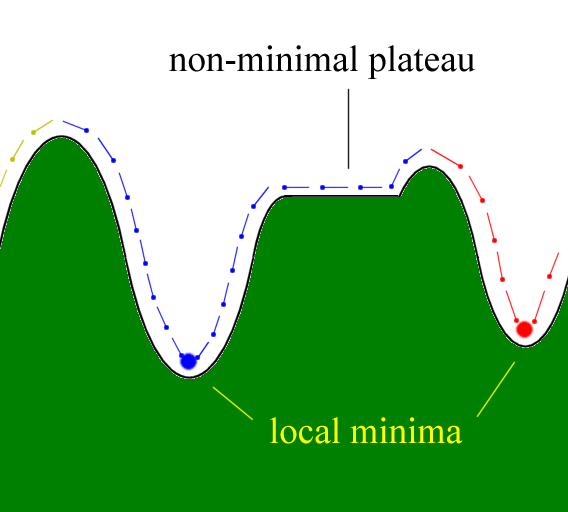
\includegraphics[height=6cm]{segmentation/segmentation-watershed-rainfallingconcept-a.png}}%
	%
	\hspace{4mm}%
	%
	\subfigure[The division into catchment basins]
	{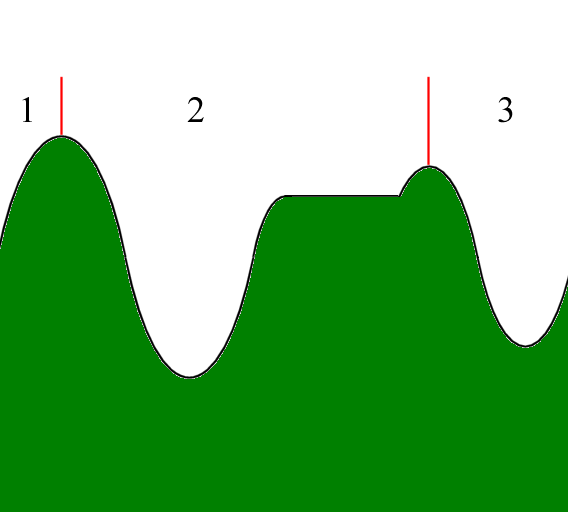
\includegraphics[height=6cm]{segmentation/segmentation-watershed-rainfallingconcept-b.png}}%
\caption{The rainfalling concept of the watershed transform}
\label{fig:segmentation-watershed-rainfallingconcept}
\end{stusubfig}
%---

%---
\begin{stusubfig}{p}
	\subfigure[Beginning the flooding]
	{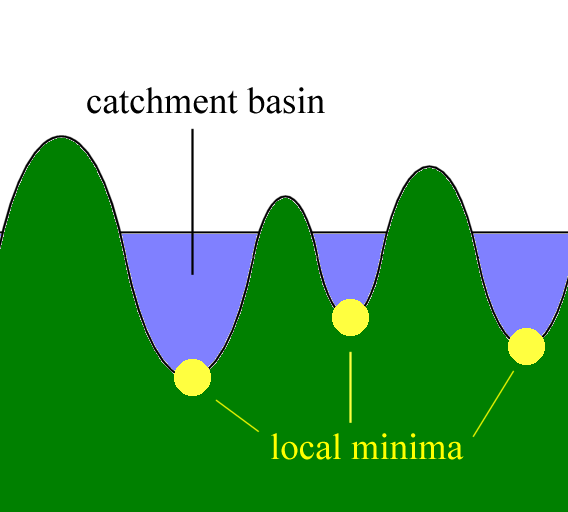
\includegraphics[height=6cm]{segmentation/segmentation-watershed-floodingconcept-a.png}}%
	%
	\hspace{4mm}%
	%
	\subfigure[Two catchment basins meet]
	{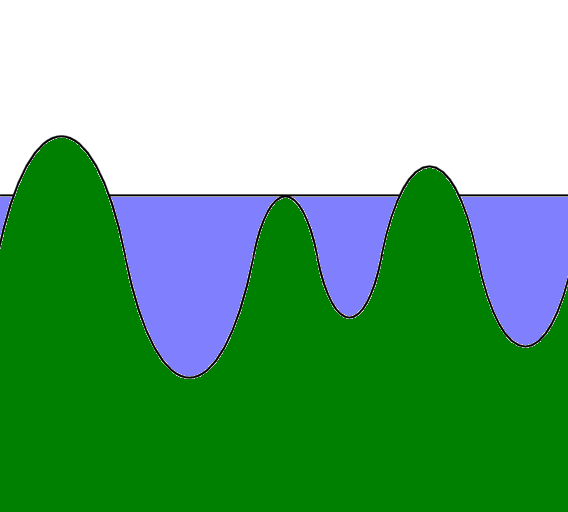
\includegraphics[height=6cm]{segmentation/segmentation-watershed-floodingconcept-b.png}}%
	%
	\hspace{4mm}%
	%
	\subfigure[Building a watershed at the join point]
	{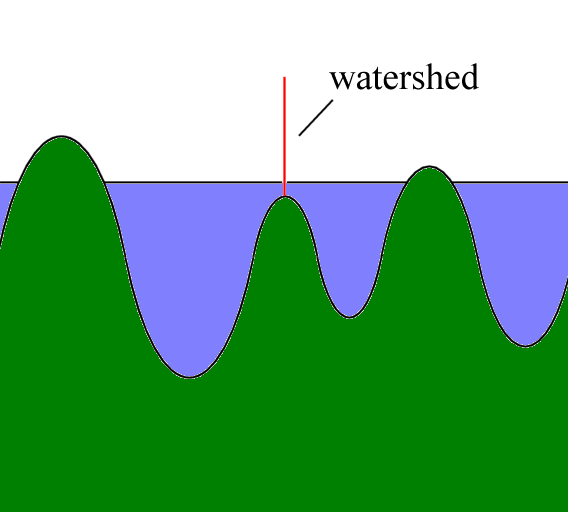
\includegraphics[height=6cm]{segmentation/segmentation-watershed-floodingconcept-c.png}}%
	%
	\hspace{4mm}%
	%
	\subfigure[The division into catchment basins]
	{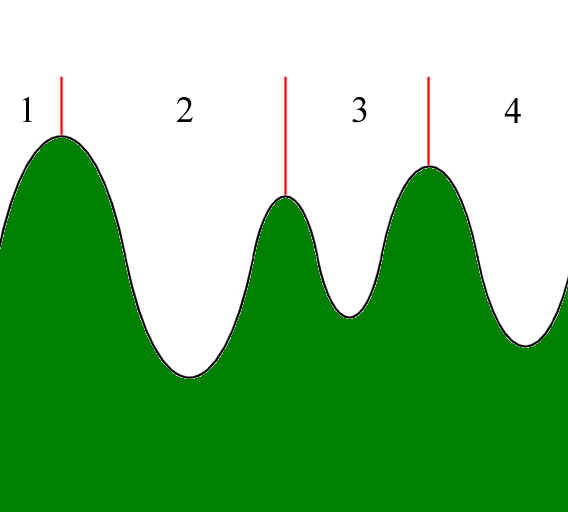
\includegraphics[height=6cm]{segmentation/segmentation-watershed-floodingconcept-d.png}}%
\caption{The flooding concept of the watershed transform}
\label{fig:segmentation-watershed-floodingconcept}
\end{stusubfig}
%---

\subsection{Segmenting Grey-Scale Images}
\label{subsec:segmentation-watershed-greyscale}

The watershed transform is commonly thought of not in the abstract terms just described, but as an image segmentation method. In particular, it is often used to segment grey-scale images. This requires a conceptual mapping that lets us view grey-scale images as landscapes. For example, we can view a 2D, grey-scale image $I$ as a height map (see Figure~\ref{fig:segmentation-watershed-landscapeanalogy}), where the grey value of the image at coordinates $(x,y)$ gives us the height of the landscape at that point. An analogous mapping can be made in higher dimensions (and specifically in three dimensions), although this is harder to visualize. The regions produced by applying an image algorithm for a watershed transform correspond to the catchment basins of the discrete landscape to which the image corresponds (see Figure~\ref{fig:segmentation-watershed-regionbasincorrespondence}).

%---
\stufigex{height=8cm}{segmentation/segmentation-watershed-landscapeanalogy.png}{The landscape analogy -- viewing a 2D image as a height map}{fig:segmentation-watershed-landscapeanalogy}{p}
%---

% TODO: fig-segmentation-watershed-regionbasincorrespondence

A variety of different watershed image algorithms are possible (e.g.~\cite{bieniek00,meijster98,osma-ruiz06,rambabu07,stoev00}), but I will focus on Meijster and Roerdink's rainfalling method described in \cite{meijster98}, not least because the ideas behind it translate across to my rainfalling algorithm for the waterfall transform described in \S\ref{subsubsec:segmentation-waterfall-myalgorithm}.

\subsubsection{Meijster and Roerdink's Rainfalling Watershed Algorithm}

\paragraph{Definitions}

For the purposes of this algorithm, we define an image to be a function $I: \Omega_{\subset \mathbb{Z}^n} \to \mathbb{Z}$ that maps elements of the domain $\Omega$ to integer grey values. (For instance, a $2$-dimensional $512 \times 512$ image could be defined to have domain $\Omega = \{(x,y) : 0 \le x,y < 512\}$.) A pixel $\mathbf{p} \in \Omega$ is defined to have height $I(\mathbf{p})$ and neighbour set $N(\mathbf{p})$, according to some implementation-defined notion of neighbourhood: usually neighbourhood is defined so that pixels are either 4- or 8-connected in 2D, and 6- or 26-connected in 3D (see Figure~\ref{fig:segmentation-watershed-connectivity}).

% TODO: fig:segmentation-watershed-connectivity

A singular minimum of an image is a point whose neighbours are all strictly higher than it. Formally, $\mathbf{p}$ is a singular minimum iff $\forall \mathbf{p'} \in N(\mathbf{p}) \cdot f(\mathbf{p'}) > f(\mathbf{p})$. A plateau of an image is a maximal set of two or more connected pixels of equal altitude. A minimal plateau is a plateau from which it is impossible to descend, and a non-minimal plateau is the opposite. Together, the singular minima and minimal plateaux of an image form the local minima of the image.

\paragraph{Overview} The approach taken by rainfalling algorithms for the watershed transform, as noted above, is to find a path of steepest descent from each point in the landscape to a local minimum in the landscape (the base of a catchment basin). This is complicated by the fact that there may be non-minimal plateaux (flat areas) in the image: if water were dropped on a pixel in the middle of a non-minimal plateau, the direction in which it would run off would be unclear. To circumvent this problem, the Meijster/Roerdink algorithm starts by transforming the image to make sure every non-minimal pixel has a lower neighbour, thus forming what is known as a lower-complete image. The rest of the algorithm is then split into two stages: in the first stage, each pixel is assigned an arrow pointing to one of its lowest neighbours, and in the second stage, these arrows are followed to find the local minimum associated with each pixel. Each local minimum has a catchment basin, which is defined as all the pixels whose paths of steepest descent lead to it. It is worth observing that points can have more than one path of steepest descent (see Figure~\ref{fig:segmentation-watershed-steepestdescent}): the decision of which one to follow for each point depends on how the arrows are assigned. Different choices lead to subtly different results, and it is important that arrows are at the very least assigned deterministically, so that the results don't vary from one run of the algorithm to the next.

%---
\stufigex{height=7cm}{segmentation/segmentation-watershed-steepestdescent.png}{The flow direction at a point is ambiguous if it has more than one path of steepest descent}{fig:segmentation-watershed-steepestdescent}{p}
%---

\paragraph{The Lower-Complete Transformation}

The lower-complete transformation described in \cite{meijster98} essentially works by raising all plateau pixels by their distance from the edge of their plateau (see Figure~\ref{fig:segmentation-watershed-plateau}(a)). Doing this na\"ively doesn't work in the general case, because it can change the ordering of the plateau pixels with respect to the other pixels in the image (see Figure~\ref{fig:segmentation-watershed-plateau}(b)). The solution is to find the maximum amount by which a plateau pixel should be raised, and multiply all pixels by that before raising any plateau pixels: this has the effect of spreading the landscape heights out to accommodate the new altitudes in the middle (see Figure~\ref{fig:segmentation-watershed-plateau}(c)).

The lower-complete transformation can be implemented straightforwardly using a breadth-first search (see Listing~\ref{code:segmentation-watershed-lowercomplete}). The results of the transformation are illustrated in Figure~\ref{fig:segmentation-watershed-example}: an example image is shown in (a), and the result of making it lower-complete is shown in (b).

%---
\begin{stusubfig}{p}
\subfigure[The `intuition' is to raise plateau pixels by their distance from the edge]
	{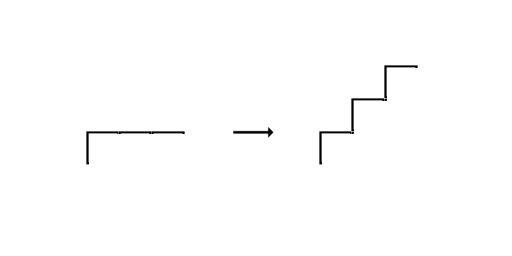
\includegraphics[width=.45\linewidth]{segmentation/segmentation-watershed-plateau-a.png}}%
	%
	\hspace{4mm}%
	%
	\subfigure[Doing this na\"ively can change the height ordering of the pixels in the image]
	{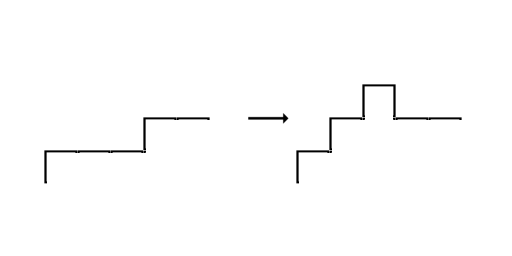
\includegraphics[width=.45\linewidth]{segmentation/segmentation-watershed-plateau-b.png}}%
	%
	\hspace{4mm}%
	%
	\subfigure[This can be fixed by spreading the landscape out prior to raising the pixels]
	{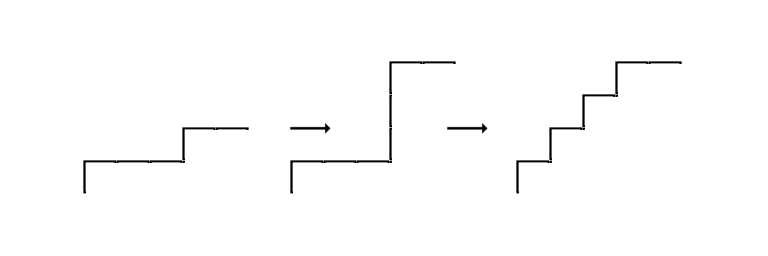
\includegraphics[width=.45\linewidth]{segmentation/segmentation-watershed-plateau-c.png}}%
\caption{A solution to the non-minimal plateau problem}
\label{fig:segmentation-watershed-plateau}
\end{stusubfig}
%---

%---
\begin{stusubfig}{p}
	\subfigure[The original image]{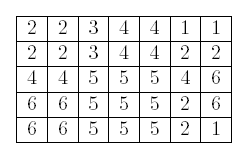
\includegraphics[height=4cm]{segmentation/segmentation-watershed-example-a.png}}%
	%
	\hspace{4mm}%
	%
	\subfigure[The lower-complete image]{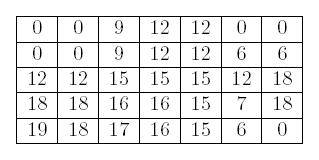
\includegraphics[height=4cm]{segmentation/segmentation-watershed-example-b.png}}%
	%
	\hspace{4mm}%
	%
	\subfigure[The arrows on each pixel]{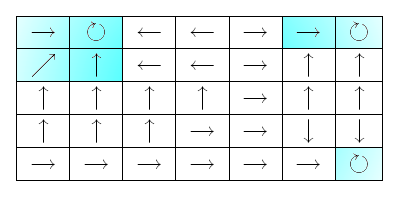
\includegraphics[height=4cm]{segmentation/segmentation-watershed-example-c.png}}%
	%
	\hspace{4mm}%
	%
	\subfigure[The final labelling]{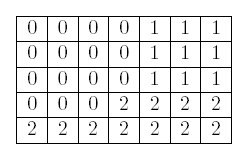
\includegraphics[height=4cm]{segmentation/segmentation-watershed-example-d.png}}%
\caption{An example illustrating the stages of the Meijster/Roerdink watershed algorithm}
\label{fig:segmentation-watershed-example}
\end{stusubfig}
%---

%---
\begin{stulisting}[p]
\caption{The Lower-Complete Transformation}
\label{code:segmentation-watershed-lowercomplete}
\begin{lstlisting}[style=Default]
function build_lower_complete
: (image : Image<$\Omega,\mathbb{Z}^+$>) $\to$ Image<$\Omega,\mathbb{Z}^+$>

	var lc : Image<$\Omega,\mathbb{Z}^+$>;
	var queue : Queue<PixelCoords>;

	// Initialise the queue with pixels that have a lower neighbour.
	for each p : PixelCoords $\in$ N(p)
		lc(p) := 0;
		for each neighbour : PixelCoords $\in$ N(p)
			if image(neighbour) < image(p) then
				queue.push(p);
				// To prevent it being queued twice.
				lc(p) := -1;
				break;

	// Compute a function which indirectly indicates the amount by which
	// we need to raise the plateau pixels (see the paper by Meijster and
	// Roerdink for more details).
	var p : PixelCoords;
	var dist : int(1);
	var marker : PixelCoords(-1,-1);
	queue.push(marker);
	while not queue.empty()
		p := queue.pop();
		if p = marker then
			if not queue.empty() then
				queue.push(marker);
				dist := dist + 1;
		else
			lc(p) := dist;
			for each neighbour : PixelCoords $\in$ N(p)
				// If the neighbouring pixel is at the
				// same altitude and has not yet been
				// processed.
				if image(neighbour) = image(p) and lc(neighbour) = 0 then
					queue.push(neighbour);
					// To prevent it being queued twice.
					lc(neighbour) := -1;
	
	// Compute the final lower-complete function. Note that at this point,
	// dist holds the amount by which we want to multiply the base image.
	for each p : PixelCoords $\in$ $\Omega$
		if lc(p) $\ne$ 0 then
			lc(p) := dist $\times$ image(p) + lc(p) - 1;

	return lc;
\end{lstlisting}
\end{stulisting}
%---

\paragraph{Arrow Assignment}

The remainder of the algorithm is designed to calculate paths of steepest descent for each point in the image. Evidently the na\"ive approach of finding a steepest path for each point in turn would be computationally costly, but this is unnecessary as the problem of finding steepest paths exhibits optimal substructure. Because of this, it suffices to assign an arrow to each pixel to indicate the direction of a steepest path through that pixel and then follow the arrows to find steepest paths for each pixel.

The arrow assignment process works as follows. Firstly, one of the pixels in each minimal plateau is chosen as a canonical element of that plateau. For each pixel, an arrow is then assigned according to its type:
%
\begin{enumerate}
\item If the pixel is a singular minimum, or the canonical element of a minimal plateau, then its arrow is a self-loop.
\item If the pixel is a non-canonical element of a minimal plateau, then its arrow points directly to the canonical element of the plateau.
\item The arrow of any other pixel points to a lowest neighbour of that pixel.
\end{enumerate}

The implementation (see Listing~\ref{code:segmentation-watershed-arrowassignment}) uses Tarjan's disjoint-set forest data structure (see Appendix~\ref{?}). The idea is to combine all the minimum points into their respective local minima using this data structure, and make all the other non-minimal points point to one of their lower neighbours. We also take the opportunity to numerically label all the canonical points of minimal plateaux during this phase of the process. The results of the arrow assignment are shown in Figure~\ref{fig:segmentation-watershed-example}(c).

%---
\begin{stulisting}[p]
\caption{Arrow Assignment}
\label{code:segmentation-watershed-arrowassignment}
\begin{lstlisting}[style=Default]
function construct_arrows
: (lc : Image<$\Omega,\mathbb{Z}^+$>) $\to$ (Image<$\Omega$,PixelCoords>, Image<$\Omega,\mathbb{Z}^+$>)

	var arrows : Image<$\Omega$,PixelCoords>;
	var labels : Image<$\Omega,\mathbb{Z}^+$>;

	// Add all the minimum points to a disjoint set forest.
	var labelCount : int(0);
	var minima : DisjointSetForest<PixelCoords>;
	for each p : PixelCoords $\in \Omega$
		if lc(p) = 0 then
			labels(p) := labelCount;
			labelCount := labelCount + 1;
			minima.add_node(p);

	for each p : PixelCoords $\in \Omega$
		if lc(p) = 0 then
			// Union any neighbouring minimum points into the same local minimum.
			for each neighbour : PixelCoords $\in$ N(p)
				if lc(neighbour) = 0 then
					minima.union_nodes(labels(p), labels(neighbour));
		else
			// Find a lowest neighbour and make this point's arrow point to it.
			var lowestNeighbour : PixelCoords(-1,-1);
			var lowestNeighbourValue : int($\infty$)
			for each neighbour : PixelCoords $\in$ N(p)
				if lc(neighbour) < lowestNeighbourValue then
					lowestNeighbour := neighbour;
					lowestNeighbourValue := lc(neighbour);
			// There will always be a lowest neighbour here since the function's lower-complete.
			arrows(p) := lowestNeighbour;

	// Assign new labels to the canonical points of the regional minima and make
	// the arrows of the non-canonical points point to them.
	labelCount := 1;
	for each p : PixelCoords $\in \Omega$
		if lc(p) $\ne$ 0 then continue
		var root : int := minima.find_set(labels(p));
		if root = labels(p) then
			// This is a canonical point.
			arrows(p) := p;
			labels(p) := labelCount;
			labelCount := labelCount + 1;
		else
			arrows(p) := minima.value_of(root);

	return (arrows, labels);
\end{lstlisting}
\end{stulisting}
%---

\paragraph{Labelling}

Once arrows have been assigned to all the pixels in the image, the paths they form from each pixel to a local minimum are followed and each pixel is assigned the label of the appropriate local minimum (see Listing~\ref{code:segmentation-watershed-labelling}). The process can be made more efficient by using path compression when following a path to a minimum (i.e.~we make all the arrows on the path point to the minimum once we've found it). This bears some similarities to the way disjoint-set forests are implemented (see Appendix~\ref{?}). The output of Meijster/Roerdink algorithm is a labelled image, as shown in Figure~\ref{fig:segmentation-watershed-example}(d). It is thus an algorithm which outputs catchment basins rather than watershed lines.

%---
\begin{stulisting}[p]
\caption{Labelling}
\label{code:segmentation-watershed-labelling}
\begin{lstlisting}[style=Default]
function resolve_all
: (arrows : Image<$\Omega$,PixelCoords>; labels : ref Image<$\Omega,\mathbb{Z}^+$>) $\to \emptyset$

	for each p : PixelCoords $\in \Omega$
		resolve_pixel(p, arrows, labels)

function resolve_pixel
: (p : PixelCoords; arrows : Image<$\Omega$,PixelCoords>; labels : ref Image<$\Omega,\mathbb{Z}^+$) $\to$ PixelCoords

	var parent : PixelCoords := arrows(p);
	if parent $\ne$ p then
		parent := resolve_pixel(parent, arrows, labels);
		labels(p) := labels(parent);
	return parent;
\end{lstlisting}
\end{stulisting}
%---

\subsection{Segmenting CT Images}

Computerised tomography (CT) is (as of the time of writing) a widely-used medical imaging modality that provides doctors with a non-invasive way to see inside their patients without needing to resort to exploratory surgery \cite{?}. CT images can be segmented using the type of grey-scale image watershed algorithm just described, but a number of issues must first be tackled in order to obtain desirable results.

\subsubsection{Smoothness}

A key issue which arises when applying the watershed to CT images is their lack of smoothness (especially in the presence of noise). The images have many local minima, most of them spurious: this is analogous to working with a highly pock-marked landscape (see Figure~\ref{fig:segmentation-watershed-pockmarkedlandscape}). Such a landscape will have many catchment basins; running a watershed algorithm on a non-smooth image will thus greatly over-segment it (each minor dimple in the landscape gets treated as a separate catchment basin).

% TODO: fig:segmentation-watershed-pockmarkedlandscape

The solution lies partly in smoothing the original image (a pre-processing step), and partly in merging the large number of small regions generated by the watershed algorithm together into larger regions with more semantic meaning (a post-processing step for which we use the waterfall transform, described later). The goal in smoothing the watershed input is to remove spurious local minima whilst preserving important semantic information in the image. In particular, it is important to try and preserve boundaries between adjacent features, which may not be as pronounced as we would prefer even at the best of times. The canonical smoothing approach for images where semantic information is less important is to pass the image through a Gaussian filter: this is not appropriate in this instance, because it uniformly blurs the image (including the boundaries in which we are interested), but more appropriate edge-preserving filters described later in this section are fundamentally adaptations of a Gaussian filter, so the Gaussian is described first.

\paragraph{Gaussian Filtering}

Gaussian filtering (also called Gaussian blurring) is essentially a form of weighted pixel averaging based on a discrete approximation to the n-dimensional version of the Gaussian (normal) distribution (where n is the dimension of the image we're blurring). The 1D Gaussian is defined as:
%
\[
g_\sigma^1(x) = \frac{1}{\sigma\sqrt{2\pi}} \exp \frac{-x^2}{2\sigma^2}
\]
%
Its 2D version\footnote{The 3D version can be obtained analogously as $g_\sigma^3(x,y,z) = g_\sigma^1(x) \times g_\sigma^1(y) \times g_\sigma^1(z)$.} can be obtained by multiplying a 1-D Gaussian in the x direction with one in the y direction:
%
\[
g_\sigma^2(x,y) = g_\sigma^1(x) \times g_\sigma^1(y) = \frac{1}{2\pi\sigma^2} \exp \left( -\frac{x^2+y^2}{2\sigma^2} \right)
\]
%
The graph of the 1D Gaussian is the familiar bell curve; the 2D version is a bell-shaped surface (see Figure~\ref{fig:segmentation-watershed-gaussian2d}).

%---
\stufigex{height=8cm}{segmentation/segmentation-watershed-gaussian2d.png}{The 2D Gaussian is a bell-shaped surface}{fig:segmentation-watershed-gaussian2d}{p}
%---

Using this for image blurring involves forming a symmetric mask (see Figure~\ref{fig:segmentation-watershed-gaussianmask}) from the values of $g_\sigma^2(x,y)$ at discrete points in a grid centred at the origin (e.g.~for a 3x3 mask, we should calculate $g_\sigma^2$ at $(-1,-1), (0,-1), (1,-1), \ldots, (0,0), \ldots, (1,1)$). The mask then needs to be normalized by dividing by the sum of all the values in it (this is done to ensure that regions of uniform intensity in the image will be unaffected by smoothing). This procedure can be used to generate masks of any size.

%---
\begin{figure}[p]
\begin{center}
\begin{tabular}{|c|c|c|}
\hline
0.0585 & 0.0965 & 0.0585 \\
\hline
0.0965 & 0.1592 & 0.0965 \\
\hline
0.0585 & 0.0965 & 0.0585 \\
\hline
\end{tabular}%
$\;\; \longrightarrow \;\;$%
\begin{tabular}{|c|c|c|}
\hline
0.0751 & 0.1238 & 0.0751 \\
\hline
0.1238 & 0.2042 & 0.1238 \\
\hline
0.0751 & 0.1238 & 0.0751 \\
\hline
\end{tabular}
\end{center}
\caption{As an example, we'll calculate a 3x3 mask for the 2D Gaussian $g_1^2(x,y)$ (i.e. the Gaussian with standard deviation $\sigma = 1$). First we calculate the values of $g_1^2(x,y)$ at the grid points (i.e. we calculate $g_1^2(-1,-1), \ldots, g_1^2(1,1)$) to give us the unnormalized mask (left); then, we normalize it by dividing through by the sum of all the values in the mask to give the final result (right).}
\label{fig:segmentation-watershed-gaussianmask}
\end{figure}
%---

The actual blurring is performed by \emph{convolving} an image $I$ with the mask to form a new image $I'$. Letting $M_\sigma^{3,3}$ be the 3x3 mask, this is written as $I' = I \otimes M_\sigma^{3,3}$. Convolution means overlaying the mask on each pixel of the image in turn, multiplying the value of each pixel in the mask by the value of the pixel beneath it, summing the results and using the value thus obtained as the value of the centre pixel in the blurred image. For the 3x3 mask with $\sigma = 1$, this means that:
%
\begin{eqnarray*}
I'(x,y)
& = & 0.0751 \times (I(x-1,y-1) + I(x+1,y-1) + I(x-1,y+1) + I(x+1,y+1)) \; + \\
&   & 0.1238 \times (I(x,y-1) + I(x,y+1) + I(x-1,y) + I(x+1,y)) \; + \\
&   & 0.2042 \times I(x,y)
\end{eqnarray*}
%
This begs the question of what happens when the mask is placed on one of the border pixels of the image (i.e.~such that part of it is outside the image). The simplest way to deal with this is to perform the weighted sum with the pixels that are in range, and then normalize by dividing by the sum of the mask values used. For instance, using this scheme we would have:
%
\[
I'(0,1) = \frac{0.0751 \times (I(1,0) + I(1,2)) + 0.1238 \times (I(0,0) + I(0,2) + I(1,1)) + 0.2042 \times I(0,1)}{2 \times 0.0751 + 3 \times 0.1238 + 0.2042}
\]

\paragraph{Edge-Preserving Filters}

Gaussian filtering is very good at smoothing an image (see Figure~\ref{fig:segmentation-watershed-smoothedimage}), but it isn't generally sufficient as the sole pre-processing filter for image segmentation because it uniformly blurs the image. This makes the image smoother, but if we smooth it enough to make it suitable for input to the watershed, we often end up destroying fine detail in which we're interested (e.g.~boundaries between organs, as mentioned previously). For any application, this would cause problems, but for medical applications it is unacceptable. The solution is to be selective about how much blurring we do in different parts of the image: specifically, we want to blur a lot in areas of little or no interest, and blur a minimal amount (or not at all) near features of interest, such as edges between organs. Each of the following two approaches described aims to accomplish this.

% TODO: fig:segmentation-watershed-smoothedimage

\subparagraph{Spatially-Variant Gaussian Filtering}

Spatially-variant Gaussian filtering (SVGF) is a simple technique I developed to perform non-uniform Gaussian blurring. The essence of the idea is to use a Gaussian filter whose standard deviation varies with its location in the image. High standard deviations cause greater smoothing, whilst a filter with a low standard deviation smoothes less strongly. The key is to ensure that the filter has a high standard deviation away from suspected edges, and a low standard deviation when near to them. This requires two things: an estimate of where the interesting edges in the image lie (obviously we don't know where they are exactly: this is effectively what we're trying to determine when segmenting the image) and a mapping from the edge estimate image to the space of standard deviations (i.e.~$\mathbb{R}^+$). The gradient magnitude of the original image (after initial smoothing with a simple Gaussian filter as described above) provides a suitable edge estimate, but the mapping requires a bit more thought.

A suitable mapping function must map high values in the edge estimate image (representing the higher estimated likelihood of an edge at that location) to a low standard deviation (thus avoiding blurring the edges) and low values to a high standard deviation (thus maximising the blurring away from the edges). In practice, we want to avoid blurring if the edge estimate for a pixel is anything other than negligible: there needs to be a sharp falloff as the edge estimate for a pixel gets bigger, so a linear decrease in $\sigma$ values won't suffice.

This still gives us a wide choice of mapping functions, but experiments showed that a sigmoid function works well in practice. For example, consider an 8-bit edge estimate image whose values range from $0$ (minimal likelihood of an edge) to $255$ (maximal likelihood). The canonical sigmoid function is given by:
%
\[
y = \frac{1}{1 + e^{-x}}
\]
%
We want to transform it into a sigmoid function which starts high at $x = 0$ and rapidly drops off to a low level. To do this, we start by deciding on the points on the shape of the normal sigmoid curve to which we want $f_1 = 0$ and $f_2 = 255$ to map (for example, mapping $f_1$ to $x_1 = 6$ and $f_2$ to $x_2 = -100$ works well in this case). We then decide on the maximum and minimum values $y_h$ and $y_\ell$ we wish our sigmoid curve to take (here, $y_h = 8$ and $y_\ell = 0$ are sensible values). Finally, we calculate the required function as follows:
%
\begin{eqnarray*}
s_x & = & (f_2 - f_1)/(x_2 - x_1) \\
o_x & = & f_1/s_x - x_1 \\
s_y & = & y_h - y_\ell \\
o_y & = & y_\ell \\
y & = & s_y/(1 + \exp(-x/s_x + o_x)) + o_y
\end{eqnarray*}
%
A suitable mapping function for the 8-bit edge estimate image is thus
%
\[
y = \frac{8}{1 + \exp(106x/255 - 6)},
\]
%
a function which starts off at nearly $8$ when $x = 0$, then drops off rapidly to nearly zero at around $x = 30$ (see Figure~\ref{fig:segmentation-watershed-sigmoid}).

%---
\stufigex{height=10cm}{segmentation/segmentation-watershed-sigmoid.png}{An example sigmoid function that maps the edge estimate at a pixel to the standard deviation of the Gaussian filter to apply there}{fig:segmentation-watershed-sigmoid}{p}
%---

SVGF works well when applied to images as part of a pipeline (see Figure~\ref{fig:segmentation-watershed-svgfpipeline}). In particular, we perform a small amount of Gaussian filtering on the image first: this blurs the image enough to remove some of the noise, but not enough to blur the important edges. The SVGF filter can then be used as a finer filter which carefully removes some of the noise remaining after applying the Gaussian.

%---
\stufigex{height=12cm}{segmentation/segmentation-watershed-svgfpipeline.png}{The SVGF pipeline}{fig:segmentation-watershed-svgfpipeline}{p}
%---

\subparagraph{Anisotropic Diffusion Filtering}

An alternative, more conventional, approach to edge-preserving image filtering is a techique known as anisotropic diffusion filtering (ADF), originally introduced by Perona and Malik in \cite{perona90}. The idea comes from the fact that solving a heat equation of the form
%
\[
\pd{I(x,y,t)}{t} = \nabla^2 I(x,y,t) \equiv \nabla \cdot \nabla I(x,y,t)
\]
%
on an image $I_0(x,y)$, by setting $I(x,y,0) = I_0(x,y)$ as the initial condition, is equivalent to convolving $I_0$ with a Gaussian of standard deviation $\sqrt{2t}$. (In other words, by finding the solution to the heat equation at a time $t_0$, we are effectively blurring the image with the corresponding Gaussian.) Perona and Malik's idea was that by replacing $\nabla I(x,y,t)$ in the equation with $C \nabla I(x,y,t)$, for some $C$, the results of solving the heat equation could be influenced to depend on where we expect the edges in the original image to be. In particular, if we assume that the gradient magnitude of the original image provides a reasonable estimate of where the edges are, then we can write $C = c(|\nabla I(x,y,t)|)$, for some function $c$, giving us the anisotropic diffusion equation
%
\[
\pd{I(x,y,t)}{t} = \nabla \cdot c(|\nabla I(x,y,t)|) \nabla I(x,y,t).
\]
%
We thereby introduce a prior expectation of where the edges to be into the equation, allowing us to influence the smoothing process so as to preserve them. The key to this is in how we specify $c$. We want the image to be blurred less where $|\nabla I|$ is large, so $c$ must yield a small value for large $|\nabla I|$ and a larger value for small $|\nabla I|$. There are obviously an infinite number of functions which would satisfy this, but an effective $c$ from the literature (and, in particular, the one used in the Insight Toolkit \cite{ITK} implementation I used) is given by
%
\[
c(|\nabla I|) = e^{-\frac{|\nabla I|^2}{2k^2}},
\]
%
where $k$ is simply a parameter used to affect the extent to which smoothing is affected by the gradient magnitude image. Overall, ADF thus takes two parameters: a time $t_0$, which indirectly specifies the standard deviation of the Gaussian used, and $k$, as just mentioned.

\subparagraph{Comparison}

TODO

\begin{itemize}
\item Compare the results of an SVGF pipeline with ADF (they're quite different)
\item Show the results of running a watershed on an image pre-processed with each
\item Mention that the impact they have on the output of the waterfall will be addressed after that has been described
\end{itemize}

\subsubsection{Features vs. Catchment Basins}

A further issue when dealing with CT images is that whilst grey-scale image watershed algorithms like the one described earlier segment the image into regions which correspond to the catchment basins of the discrete landscape associated with the image, it is unusual for these catchment basins to correspond directly to features of interest in our input image. For instance, if we're trying to segment a kidney in a CT image, there is no reason to suppose that the kidney will correspond to a catchment basin in the landscape: applying a watershed algorithm directly, therefore, will not in general yield useful results.

What we need is a way of transforming our input image into one where the features of interest correspond more directly to its catchment basins. Unfortunately there is no domain-independent solution to this (it depends on the type of image we are segmenting and the sort of features in which we're interested), but it is possible to come up with suitable transformations on a domain-by-domain basis. Our goal in the case of CT images is generally to segment things like organs. The grey value in the images tends to vary relatively slowly across individual organs and relatively quickly at their edges because of the tissue types involved (another way of saying this is that the organs tend to be homogeneous). The intuition is therefore that the value of the gradient magnitude is relatively low within organs, and relatively high at their edges (see Figure~\ref{fig:segmentation-watershed-gradientmagnitude}), so by running the watershed on the gradient magnitude image instead of the original input we can get a much better correspondence between organs and catchment basins (i.e.~a much better segmentation result). It should be noted, however, that this scheme is of less use to us when our goal is to segment inhomogeneous features like tumours.

%---
\begin{stusubfig}{p}
	\subfigure[A sample medical image (courtesy of the Churchill Hospital, Oxford)]
	{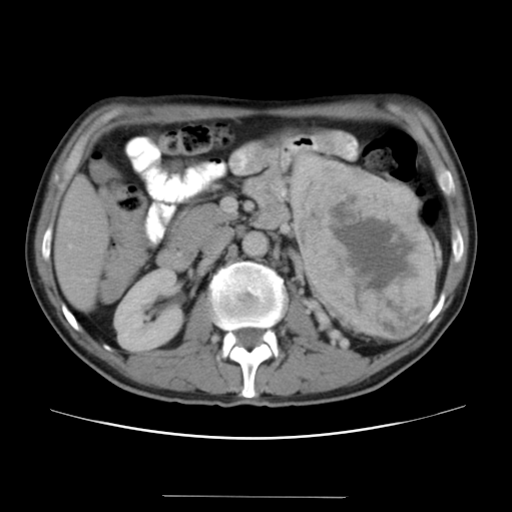
\includegraphics[width=.45\linewidth]{segmentation/segmentation-watershed-medicalimage.png}}%
	%
	\hspace{4mm}%
	%
	\subfigure[The corresponding gradient magnitude image]
	{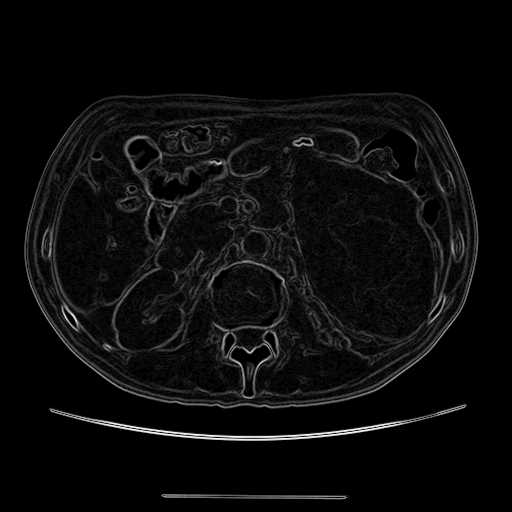
\includegraphics[width=.45\linewidth]{segmentation/segmentation-watershed-gradientmagnitudemedicalimage.png}}%
\caption{To a first approximation, the value of the gradient magnitude image is relatively low within organs, and relatively high at their edges}
\label{fig:segmentation-watershed-gradientmagnitude}
\end{stusubfig}
%---

\subsubsection{Hounsfield Units and Windowing}

A final issue to contend with when working with CT images concerns the scale used for their pixel values. The images produced by CT scanners are called Hounsfield images: these are scalar images (i.e.~each pixel value is a scalar), so all the algorithms previously described can be applied to them, but their pixel values are calibrated to a special scale, known as the Hounsfield scale (after Sir Godfrey Hounsfield, one of the pioneers of CT technology). The values, measured in Hounsfield Units (HU), are based on the radiodensity of materials with respect to water, and range from $-1024$ to $3071$. Materials which have a lower radiodensity than water have negative Hounsfield values; conversely, those with a greater radiodensity than water have positive values. On this scale, for example, air is at $-1000$ HU, whereas bone appears at $400$ HU or more. The scale is calibrated so that water itself is at $0$ HU.

Having the scanners calibrated to produce images whose pixel values are on a fixed scale with real-world meaning is extremely helpful, but in order to diagnose patients, radiologists need to be able to clearly distinguish between different types of tissue on a viewable image. Unfortunately, there is a limit to how many grey values can be distinguished by the human visual system, and the Hounsfield range is too wide ($> 4000$ distinct values) for Hounsfield images to be directly used for diagnostic purposes. (Looking at things another way, viewing a Hounsfield image directly would be equivalent to looking at an image with extremely low contrast.) For this reason, Hounsfield images are subjected to a process known as windowing before being viewed by a radiologist.

% TODO: fig:segmentation-watershed-windowing

Windowing is essentially a way of changing the brightness and contrast of the image (in particular, in a way that makes practical sense to radiologists). Rather than viewing the entire Hounsfield scale, the radiologist can select a window on the scale which is mapped to the available grey values (see Figure~\ref{fig:segmentation-watershed-windowing}). The position and size of the window are controlled by two parameters, known respectively as the \emph{window level} (L) and \emph{window width} (W). With the window set, the Hounsfield image can then be transformed into a human-viewable grey-scale image. For example, if we were working with 8-bit greyscale images (with $0$ being black and $2^8 - 1 = 255$ being white), then pixels with Hounsfield value $\le L - W/2$ would be mapped to $0$ and those with value $\ge L + W/2$ would be mapped to $255$, with pixel values in between being mapped using the formula:
%
\[
\mbox{Out} = \mbox{Round}\left( (\mbox{In} - L) \times \frac{255}{W} + 127.5 \right)
\]
%
The reason windowing is a sensible way for radiologists to control the brightness and contrast of an image (rather than just adjusting them directly) is that it allows them to focus on an interesting part of the scale. For instance, when diagnosing kidney tumours, it is common to use a window level of $40$ and a window width of $400$ in order to focus on organs made of soft tissue (like the kidneys). A window like $40/400$ would thus be referred to as a soft tissue window. Different windows are used for other types of investigation (e.g.~when looking at lung images), and it is common for appropriate window settings chosen by a radiologist to be stored with each image as meta-data.

Windowing makes a practical difference for the purposes of segmentation. In particular, it is possible to work with either the original Hounsfield image or a windowed version of it, and these yield different results. It is noticeable that segmenting a windowed image (using an appropriately chosen window, such as the one stored with the image) tends to work better in practice, in that it produces a less pronounced oversegmentation of the image (see Figure~\ref{fig:segmentation-watershed-hounsfieldvswindowed}). This may seem surprising, since there is effectively less information in the windowed image than the original, but there is a logical explanation. When the width of window chosen is greater than the width of the greyscale range, the process of windowing will map more than one Hounsfield value to the same grey-scale output (one reason why there is a loss of information involved). This has the effect of removing some of the spurious local minima in the image, which improves the resulting watershed segmentation. In short, whilst we are losing some of the information from the original Hounsfield image, the information we are losing was actually hindering the segmentation rather than helping it.

% TODO: fig:segmentation-watershed-hounsfieldvswindowed

\subsubsection{Summary}

To segment a CT image using the watershed transform, then, we first window it using appropriate window settings (generally speaking, the ones stored with the image by a radiologist) in order to obtain a more conventional grey-scale image. We next smooth it using an edge-preserving filter (as we have seen, anisotropic diffusion filtering is preferred for this step) and then pass it through a gradient magnitude filter to try and establish a reasonable correspondence between features of interest in the image and catchment basins in the discrete landscape associated with it. Finally, we run an image watershed algorithm on this smoothed, gradient magnitude image: in our case, we use the Meijster/Roerdink algorithm, which produces an image of numeric labels. As we will see in \S\ref{sec:segmentation-ipfconstruction}, this labelled image is what we need to construct the leaf layer and lowest branch layer of an IPF for the image. The remainder of the IPF will be constructed using the waterfall transform, which will now be introduced.

\afterpage{\clearpage}

%---
\section{The Waterfall Transform}

\subsection{Motivation}

The watershed transform segments a landscape into its catchment basins, but, as we have seen, this often produces a segmentation that contains far too many regions to be useful for the specific application in which we're interested (segmenting CT images, for example). In the specific context of images, pre-processing the image with an edge-preserving filter helps alleviate the problem somewhat, but fails to solve it.

One method that seeks to solve this problem is the so-called `watershed-from-markers' approach \cite{meyer90}. The idea behind this is to specify a priori that only certain local minima in the landscape are semantically interesting. Conceptually, we can do this by filling in all the non-interesting minima and keeping only the interesting ones (see Figure~\ref{fig:segmentation-waterfall-watershedfrommarkers}), although this is not how the approach tends to be implemented in practice. An example implementation can be found in e.g.~\cite{felkel01}. (Alternatively, consider an approach whereby we flood the landscape from the local minima and only add watersheds when two \emph{marked} catchment basins would otherwise meet.) We can thus constrain the watershed to produce an output with a certain number of regions in it (solving the problem of oversegmentation), provided that we can determine the local minima in which we're interested (the markers) in advance.

%---
\begin{stusubfig}{p}
	\subfigure[Placement of markers (the blue dots)]
	{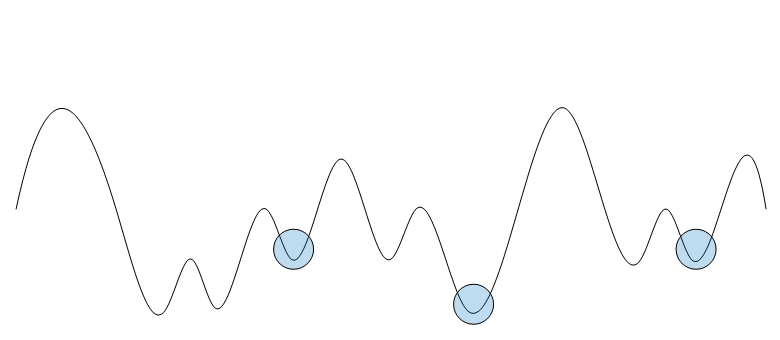
\includegraphics[width=.6\linewidth]{segmentation/segmentation-waterfall-watershedfrommarkers-a.png}}%
	%
	\hspace{4mm}%
	%
	\subfigure[After filling in the non-interesting minima]
	{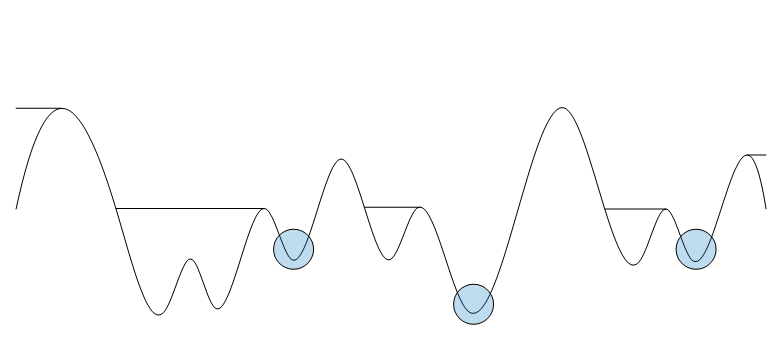
\includegraphics[width=.6\linewidth]{segmentation/segmentation-waterfall-watershedfrommarkers-b.png}}%
	%
	\hspace{4mm}%
	%
	\subfigure[After performing a watershed on the filled landscape]
	{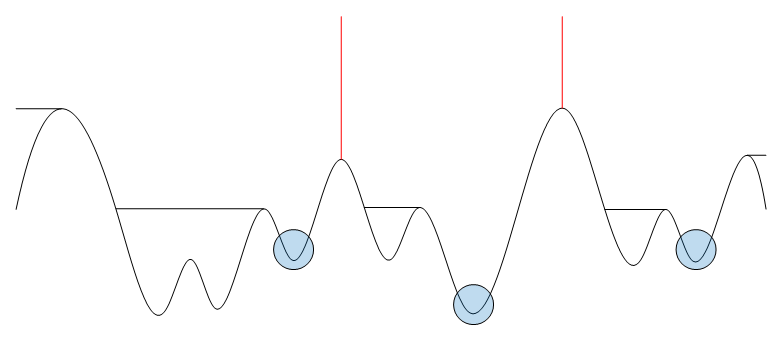
\includegraphics[width=.6\linewidth]{segmentation/segmentation-waterfall-watershedfrommarkers-c.png}}%
\caption{A conceptual view of the watershed-from-markers approach}
\label{fig:segmentation-waterfall-watershedfrommarkers}
\end{stusubfig}
%---

Marker determination can be either manual or automatic, but both approaches have their problems. In the manual approach, the user simply clicks the interesting local minima and then runs the segmentation. The downside is that the process is not only time-consuming, but non-intuitive: obtaining a desirable segmentation by selecting markers tends to involve a lot of trial-and-error. Automatic approaches are more promising: for example, we could pick the local minima associated with `the n deepest catchment basins' as our markers. The disadvantage in this case is that the results are `all or nothing': a specific automatic marker approach is unlikely to work well for all possible images, and if we get a bad result on a particular image then we have nothing to work with (we are left with a poor segmentation and no obvious way to edit it).

Whilst watershed-from-markers has been used successfully in a variety of situations \cite{?}, the issues just mentioned make it an undesirable approach to use in the context of trying to minimise the amount of user interaction necessary whilst maximising the amount possible (see Chapter~\ref{chap:motivation}). A more usable approach for our purposes is to stick with pre-processing the image as described earlier, but to post-process it afterwards to deal with the oversegmentation. This post-processing comes in the form of a hierarchical watershed-based transform, known as the waterfall.

\subsection{Concept}

The waterfall transform is a multi-pass, hierarchical segmentation method. It generates a sequence of partitions of a landscape, each coarser (i.e.~containing fewer regions) than the one preceding it. An illustration of this is Figure~\ref{fig:segmentation-waterfall-partitionsequence}, which shows the result of applying a waterfall algorithm to an example image.

% TODO: fig: segmentation-waterfall-partitionsequence

Each waterfall pass takes a partition of the landscape as input, merges some of the adjacent catchment basins together, and returns a coarser partition as its result. The input partition to the first pass is the output of an initial watershed transform on the landscape. The final partition (if we go that far) would be the whole landscape, but for most applications the regions contained in the coarsest few partitions are of little semantic interest, so the process is often terminated early.

In image terms, the waterfall helps solve the problem of oversegmentation by iteratively merging some of the regions together in a sensible way, so that regions in subsequent partitions tend to both be larger, and correspond to semantically interesting features in the image. (This will allow us to search through all the partitions to find interesting regions, as we will see in Chapter~\ref{chap:featureid}.)

\subsubsection{A Waterfall Pass}

Conceptually, each pass of the waterfall takes its input partition (Figure~\ref{fig:segmentation-waterfall-passconcept}(a)) and transforms it into a `stepped' landscape, where there is a step corresponding to each watershed boundary, with the height of the lowest pass point along that boundary (Figure~\ref{fig:segmentation-waterfall-passconcept}(b)). It then performs a watershed transform on this stepped landscape and outputs a coarser partition of the landscape as its result (Figure~\ref{fig:segmentation-waterfall-passconcept}(c)). This process can be repeated as long as the most recent partition has more than one catchment basin (Figures~\ref{fig:segmentation-waterfall-passconcept}(d) and (e)).

%---
\begin{stusubfig}{p}
	\subfigure[The initial partition output by the watershed]
	{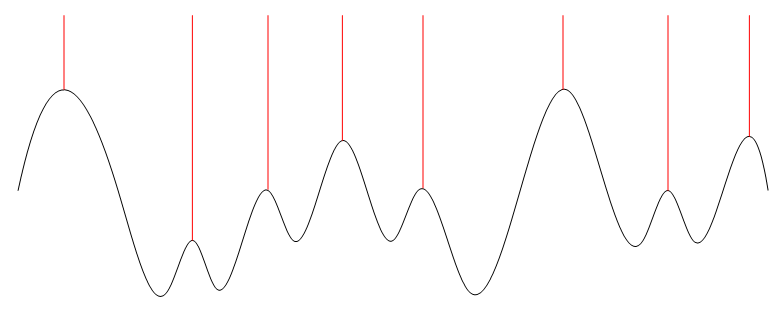
\includegraphics[width=.6\linewidth]{segmentation/segmentation-waterfall-passconcept-a.png}}%
	%
	\hspace{4mm}%
	%
	\subfigure[After transforming it into a stepped landscape]
	{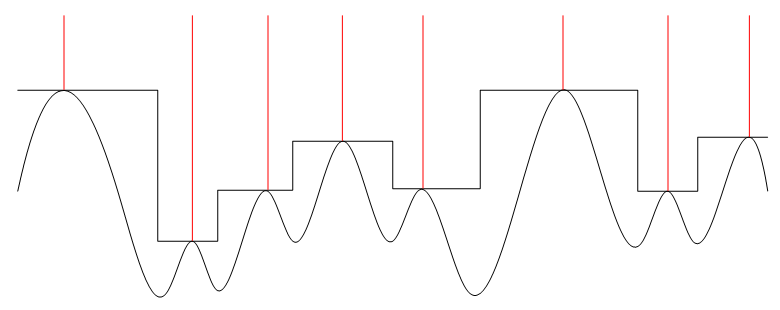
\includegraphics[width=.6\linewidth]{segmentation/segmentation-waterfall-passconcept-b.png}}%
	%
	\hspace{4mm}%
	%
	\subfigure[After performing a watershed transform on the stepped landscape]
	{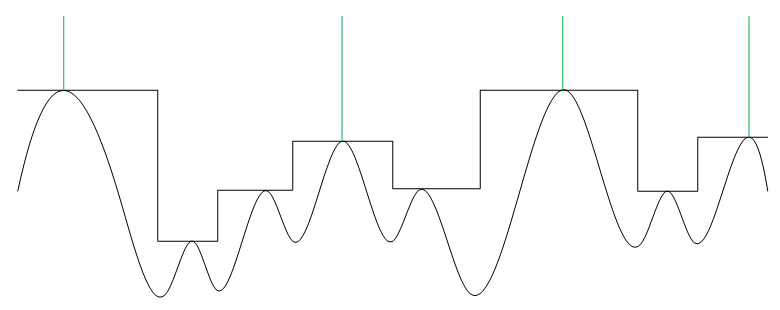
\includegraphics[width=.6\linewidth]{segmentation/segmentation-waterfall-passconcept-c.png}}%
	%
	\hspace{4mm}%
	%
	\subfigure[After the second step transformation]
	{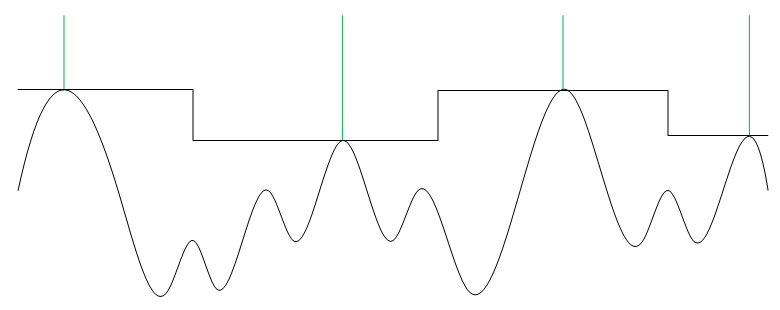
\includegraphics[width=.6\linewidth]{segmentation/segmentation-waterfall-passconcept-d.png}}%
	%
	\hspace{4mm}%
	%
	\subfigure[After performing another watershed transform]
	{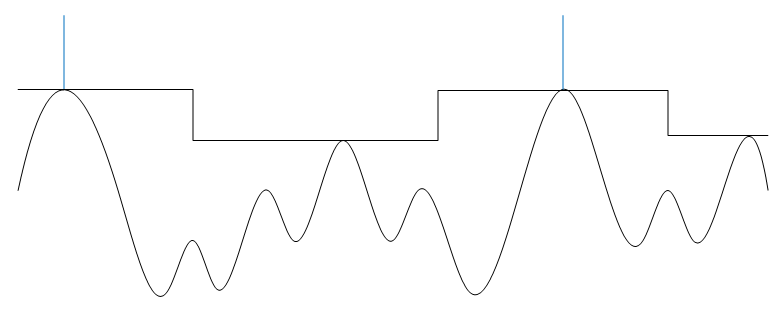
\includegraphics[width=.6\linewidth]{segmentation/segmentation-waterfall-passconcept-e.png}}%
\caption{A conceptual view of the waterfall transform}
\label{fig:segmentation-waterfall-passconcept}
\end{stusubfig}
%---

\subsection{Practical Waterfall Algorithms}

In practice, actually transforming the landscape for each waterfall pass would be a slow process and is better avoided. More practical implementations of the waterfall are possible which work on a weighted graph whose edges correspond to watershed boundaries and whose nodes correspond to regions in the input partition (in other words, the region adjacency graph of the input partition: this is illustrated in Figure~\ref{fig:segmentation-waterfall-rag}).

%---
\stufigex{height=6cm}{segmentation/segmentation-waterfall-rag.jpg}{An example image partition and its region adjacency graph. Note that this is an abstract diagram designed for explication purposes only: regions have been given arbitrary colours, and edges to the surrounding (beige) region and weights on all other edges have been omitted, in order to reduce unnecessary clutter in the image.}{fig:segmentation-waterfall-rag}{p}
%---

In fact, as shown in \cite{marcotegui05}, it actually suffices to work just on a minimum spanning tree (MST) of such a graph (see Appendix~\ref{chap:datastructures}). Each waterfall pass then takes such an MST as its input and elides appropriate edges in it (eliding an edge means combining the nodes at either end of the edge and removing the edge itself from the MST). This has the effect of merging the partition regions joined by the edges (since the nodes which are combined actually represent regions in the partition). It is worth observing in passing (because it sheds some insight on the development of the algorithms which follow) that the goal of a MST-based waterfall algorithm is only to decide which edges in the MST need to be elided: if concerns are properly separated at a code level, the issue of how this elision process takes place can be entirely ignored for the purposes of the waterfall, and different implementations can be substituted for each other with relative impunity.

The weights on the graph edges, in correspondence with the conceptual description of the algorithm given above, are the heights of the lowest pass points along the corresponding watershed boundaries. There is, however, no reason why other valuations for the graph edges cannot be used (indeed, examples are given in \cite{marcotegui05}): these generate different, non-waterfall partition hierarchies.

\subsubsection{Marcotegui's Algorithm}

Since each waterfall pass is effectively just a graph-based waterfall transform, it can be implemented using either a flooding or a rainfalling approach. The algorithm described in \cite{marcotegui05} is an example of the former. Each pass performs a flooding-based watershed transform on MSTs, consisting of the following three steps:

\begin{enumerate}

\item \emph{Determination of Local Minima}. We define a local minimum of a weighted graph G to be a connected subgraph of G whose own edges have equal weight and whose adjacent edges in G have strictly higher weights. Figure~\ref{fig:segmentation-waterfall-marcotegui-graphlocalminima} shows an example graph and its local minima. Note that the two edges with a weight of $4$ are part of the same local minimum. The first step of the algorithm consists of determining the local minima of the MST. To do this, we iterate over all the edges in the MST and flood outwards from each one to determine (a) whether it's part of a local minimum and (b) the extent of the local minimum if so.

%---
\stufigex{height=6cm}{segmentation/segmentation-waterfall-marcotegui-graphlocalminima.png}{An example graph and its local minima (drawn in red)}{fig:segmentation-waterfall-marcotegui-graphlocalminima}{p}
%---

\item \emph{Elision of Local Minima}. Having determined the local minima of the MST, we next elide all the edges in them: this is equivalent to merging minimal plateaux in a landscape into single points to which water can be considered to run down. In the original paper (and in the diagrams, for reasons of clarity), the nodes at the ends of an edge are assigned the same label, rather than the edge itself being elided, but the end result is the same. See Figure~\ref{fig:segmentation-waterfall-marcotegui-localminimaelision} for an illustration.

%---
\stufigex{height=6cm}{segmentation/segmentation-waterfall-marcotegui-localminimaelision.png}{Eliding/labelling the local minima (the edges to be elided are drawn in blue)}{fig:segmentation-waterfall-marcotegui-localminimaelision}{p}
%---

\item \emph{Propagation}. Finally, we flood out from the nodes which now represent the local minima (so-called `marker nodes') along the edges, in non-decreasing order of edge weight, starting from the edges directly adjacent to the marker nodes. Each edge considered will either join a marker node to another marker node, in which case it should be ignored (since eliding it would mean merging two catchment basins in the MST), or it will join a marker to a non-marker, in which case it should be elided. An illustration of the process is shown in Figure~\ref{fig:segmentation-waterfall-marcotegui-propagation}.

%---
\begin{stusubfig}{p}
	\subfigure[The start of the propagation]{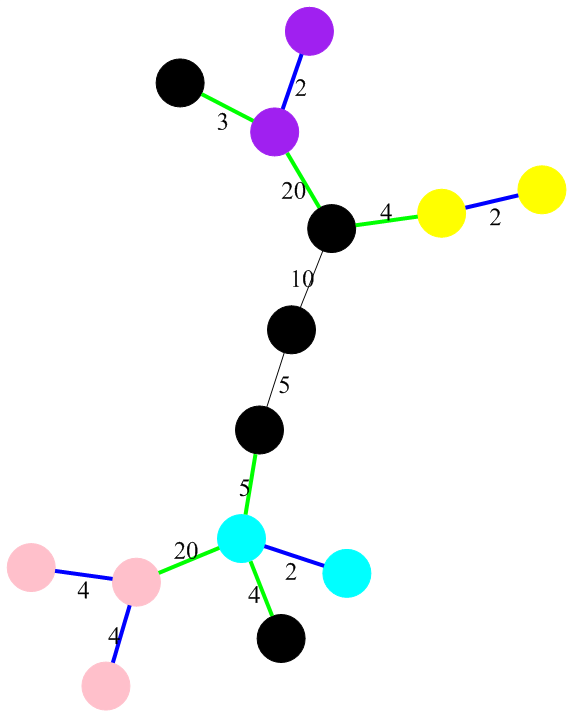
\includegraphics[width=.3\linewidth]
	{segmentation/segmentation-waterfall-marcotegui-propagation-a.png}}%
	\hspace{4mm}%
	\subfigure[The 3 edge is lowest (and elidable), so elide it]{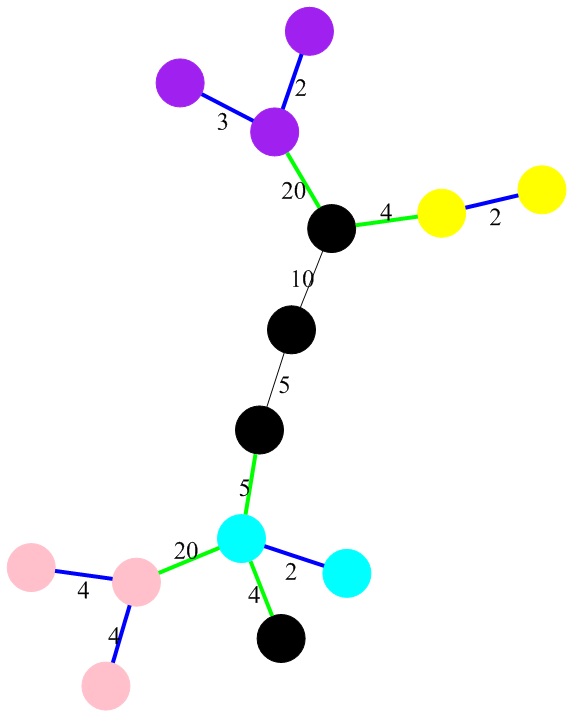
\includegraphics[width=.3\linewidth]
	{segmentation/segmentation-waterfall-marcotegui-propagation-b.png}}%
	\hspace{4mm}%
	\subfigure[A 4 edge is lowest (and elidable), so elide it]{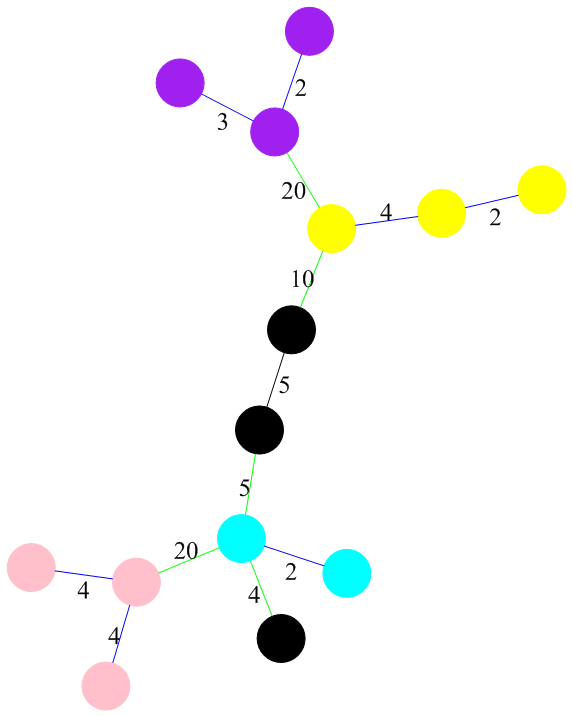
\includegraphics[width=.3\linewidth]
	{segmentation/segmentation-waterfall-marcotegui-propagation-c.png}}%
	\hspace{4mm}%
	\subfigure[The other 4 edge is lowest (and elidable), so elide it]{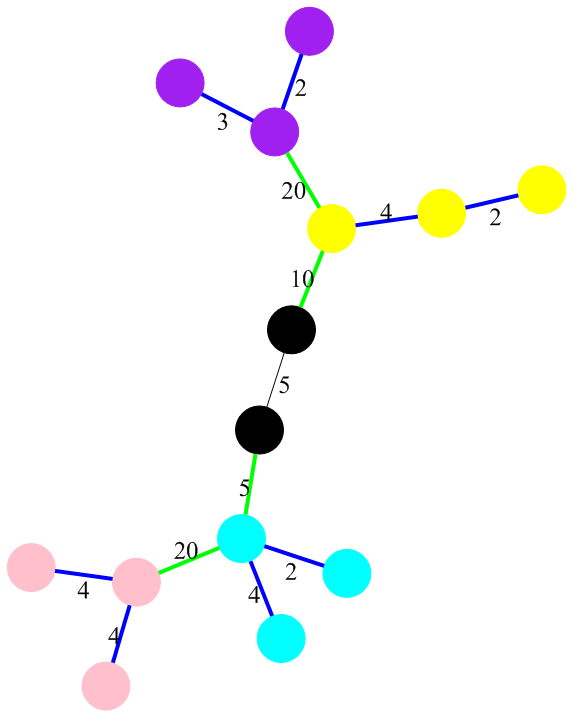
\includegraphics[width=.3\linewidth]
	{segmentation/segmentation-waterfall-marcotegui-propagation-d.png}}%
	\hspace{4mm}%
	\subfigure[The 5 edge is lowest (and elidable), so elide it]{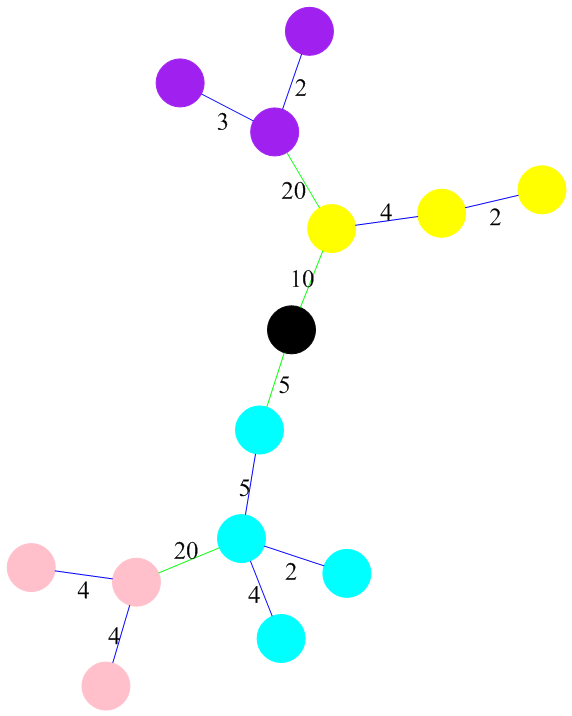
\includegraphics[width=.3\linewidth]
	{segmentation/segmentation-waterfall-marcotegui-propagation-e.png}}%
	\hspace{4mm}%
	\subfigure[The other 5 edge is lowest (and elidable), so elide it; all remaining edges will be considered in order but not elided because they are not elidable]{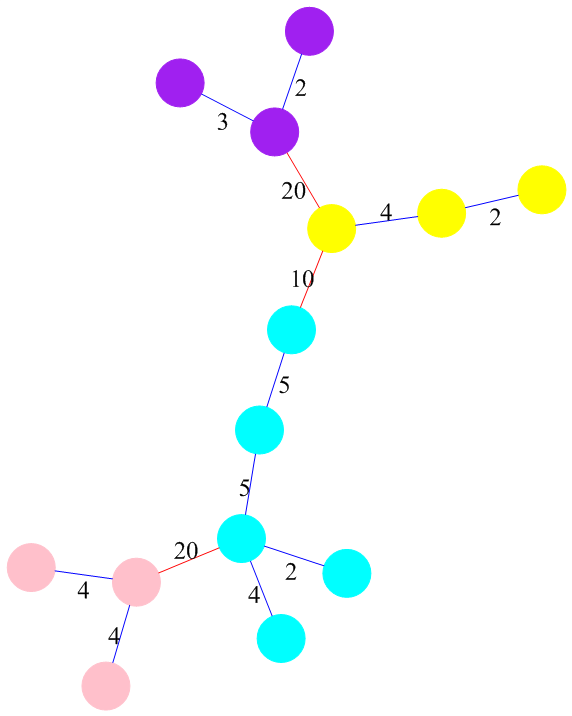
\includegraphics[width=.3\linewidth]
	{segmentation/segmentation-waterfall-marcotegui-propagation-f.png}}%
\caption{The propagation step of Marcotegui's waterfall algorithm, illustrated on the graph in \cite{marcotegui05}: blue edges are those that have already been elided, green edges are the ones currently under consideration, and red edges are those that will not be elided.}
\label{fig:segmentation-waterfall-marcotegui-propagation}
\end{stusubfig}
%---

\end{enumerate}

A more implementation-focused description of the algorithm, including code, can be found in \cite{golodetz08}. It is important to note that the order in which edges should be processed during the propagation step is not in general well-defined (note that I wrote `non-decreasing' rather than `increasing' order of edge weight above, since multiple edges under consideration can have the same weight). The `obvious' implementation of the propagation step uses a priority queue and pops a lowest adjacent edge for consideration each time: thus the next edge to be considered ends up depending fundamentally on the way the priority queue is implemented. This has significant consequences: as mentioned previously, the issue of how to handle non-minimal plateaux in a landscape is possibly the key problem to be faced when implementing a watershed-based method. Whilst it can be argued that the quality of the resulting segmentation is what is most important (in other words, as long as the end result is semantically interesting, the choice made about handling non-minimal plateaux can be somewhat arbitrary), it is nevertheless undesirable to have the segmentation output depend closely on the implementation of an internal data structure which may in principle be subject to change. I will return to this issue in the following subsections.

\subsubsection{Nicholls' Algorithm}

Marcotegui's waterfall method is fast and effective, but there are at least two aspects of it that are worth looking at. The first has just been mentioned -- the algorithm does not well-specify which edges should be elided when there are non-minimal plateaux in the MST, essentially leaving it to the implementor to make a sensible choice. I address this robustly in my algorithm below. The second is that the algorithm as defined is a general graph algorithm, even though it is actually operating on a tree: this makes implementing the waterfall a somewhat more intricate procedure than is strictly necessary and makes the code harder to understand.

This latter problem was the motivation behind the development of a simpler, tree-based waterfall algorithm by (my colleague) Chris Nicholls \cite{nicholls09}. His observation is that if an edge is not elided by a waterfall pass, it is because it is a highest edge separating two adjacent catchment basins (an alternative phrasing is that it is a highest edge on the MST path between two adjacent local minima in the MST). Instead of explicitly finding the local minima in the graph and flooding out from them, therefore, it suffices to root the MST somewhere and then work recursively up from the bottom of the tree, carefully maintaining a highest edge (a `guard' edge) guarding each local minimum encountered as we go.

%---
\begin{stusubfig}{p}
	\subfigure[Before rooting the MST]
	{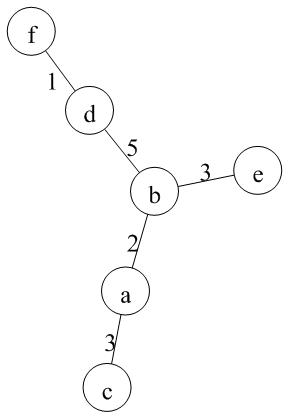
\includegraphics[height=8cm]{segmentation/segmentation-waterfall-nicholls-root-before.png}}%
	%
	\hspace{4mm}%
	%
	\subfigure[After rooting it: note the dummy root edge that gets added above the chosen root]
	{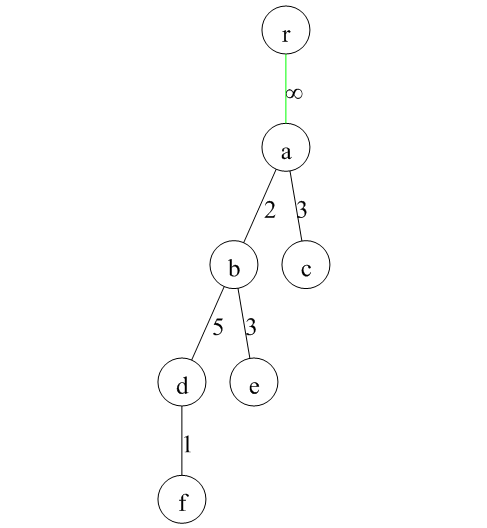
\includegraphics[height=8cm]{segmentation/segmentation-waterfall-nicholls-root-after.png}}%
\caption{Nicholls' algorithm starts by picking a node at which to root the MST and adding a dummy root edge}
\label{fig:segmentation-waterfall-nicholls-root}
\end{stusubfig}
%---

Nicholls' algorithm first roots the MST (see Figure~\ref{fig:segmentation-waterfall-nicholls-root}), adding a dummy `root edge' with a value strictly greater than the values of the edges descending from the root node (I will henceforth -- and without ambiguity -- call edges descending from a node children of the edge ascending from that node). The value chosen is unimportant, but $\infty$ or $1$ greater than the maximum value on a child edge are sensible choices. Each pass of the algorithm is then invoked on the root edge, and proceeds recursively as follows:

%-
\begin{enumerate}

\item If the current edge is a leaf edge (i.e.~it has no child edges) then it is marked as a non-guard edge.

\item Otherwise:

%--
\begin{enumerate}

\item A child edge with minimum value is chosen (if one or more of the children with minimum value is a guard edge, one of those is chosen in preference to a non-guard). This is then referred to as the `lowest child'. The value on the current edge is compared to the value on the lowest child. If its value is less than that of the lowest child, it is marked as a non-guard edge; otherwise it is marked as a guard and the lowest child is marked as a non-guard.

\item All non-guard children are now elided.

\end{enumerate}
%--

\end{enumerate}
%-

A case analysis of what is going on should prove illuminating. There are in fact only two cases to consider: either the current edge (the parent edge) isn't strictly the lowest leading out of a node, in which case at least part of the implied flow from the node is along the lowest child (see Figure~\ref{fig:segmentation-waterfall-nicholls-cases}(a)), or it is, in which case the implied flow from the node is entirely along the parent (see Figure~\ref{fig:segmentation-waterfall-nicholls-cases}(b)). In the first case, the algorithm arbitrarily assumes that all the implied flow is along the lowest child. In both cases, the various child edges are then elided (or not) accordingly. Figure~\ref{fig:segmentation-waterfall-nicholls-example} illustrates how the algorithm works on the same graph used to illustrate Marcotegui's algorithm above.

%---
\begin{stusubfig}{p}
	\subfigure[The edge under consideration is not the unique lowest edge]{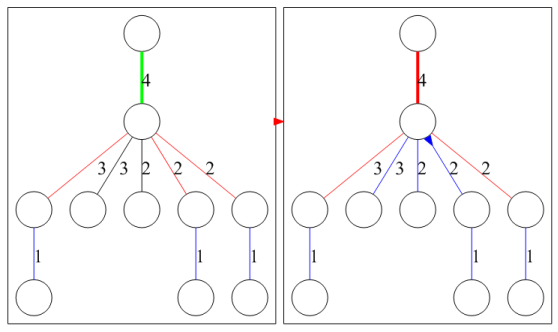
\includegraphics[height=7cm]{segmentation/segmentation-waterfall-nicholls-cases-a.png}}%
	\hspace{4mm}%
	\subfigure[The edge under consideration is the unique lowest edge]{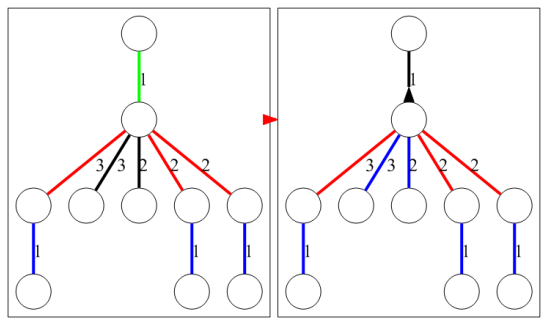
\includegraphics[height=7cm]{segmentation/segmentation-waterfall-nicholls-cases-b.png}}%
\caption{Case analysis for the recursive step of Nicholls' algorithm: black edges are non-guards, red edges are guards, blue edges are those which have been elided and the green edge is the one under active consideration. The arrow (on the node) indicates the direction in which the algorithm presumes water to flow.}
\label{fig:segmentation-waterfall-nicholls-cases}
\end{stusubfig}
%---

%---
\begin{stusubfig}{p}
	\subfigure[Level 7]{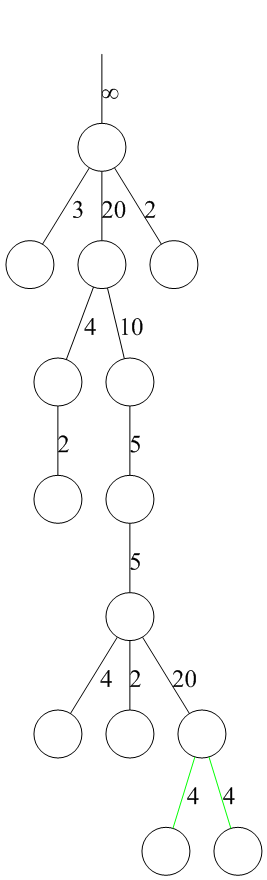
\includegraphics[width=.2\linewidth]{segmentation/segmentation-waterfall-nicholls-example-a.png}}%
	\hspace{4mm}%
	\subfigure[Level 6]{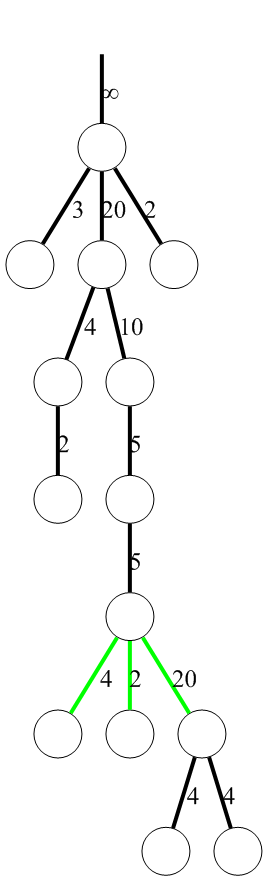
\includegraphics[width=.2\linewidth]{segmentation/segmentation-waterfall-nicholls-example-b.png}}%
	\hspace{4mm}%
	\subfigure[Level 5]{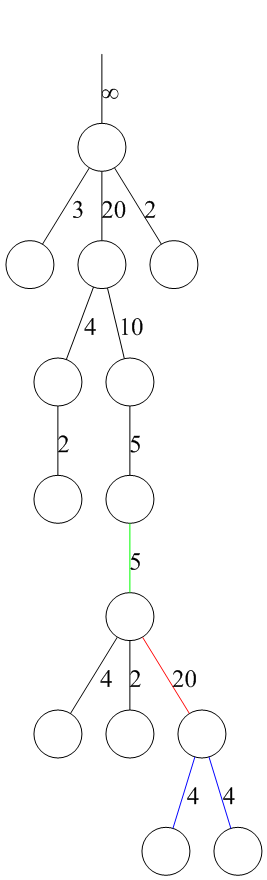
\includegraphics[width=.2\linewidth]{segmentation/segmentation-waterfall-nicholls-example-c.png}}%
	\hspace{4mm}%
	\subfigure[Level 4]{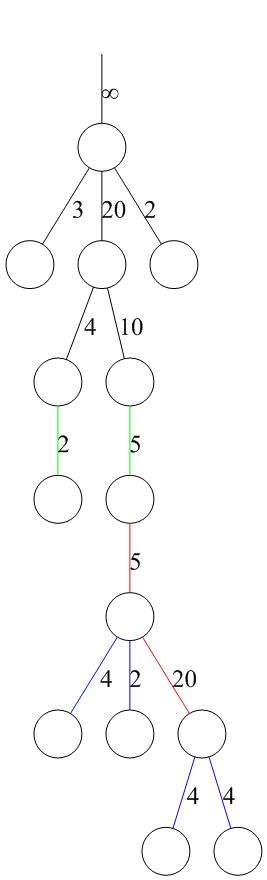
\includegraphics[width=.2\linewidth]{segmentation/segmentation-waterfall-nicholls-example-d.png}}%
	\hspace{4mm}%
	\subfigure[Level 3]{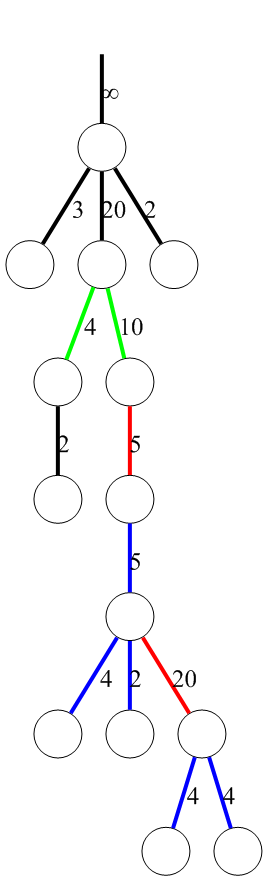
\includegraphics[width=.2\linewidth]{segmentation/segmentation-waterfall-nicholls-example-e.png}}%
	\hspace{4mm}%
	\subfigure[Level 2]{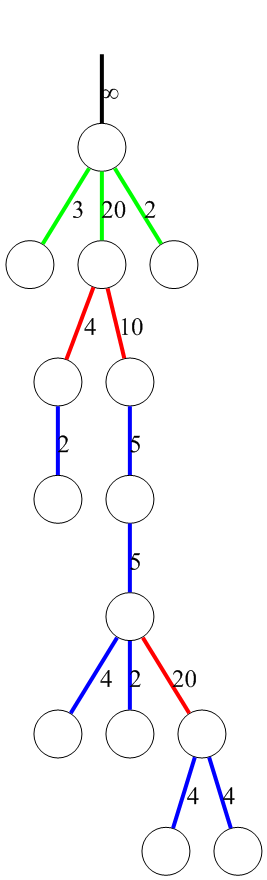
\includegraphics[width=.2\linewidth]{segmentation/segmentation-waterfall-nicholls-example-f.png}}%
	\hspace{4mm}%
	\subfigure[Level 1]{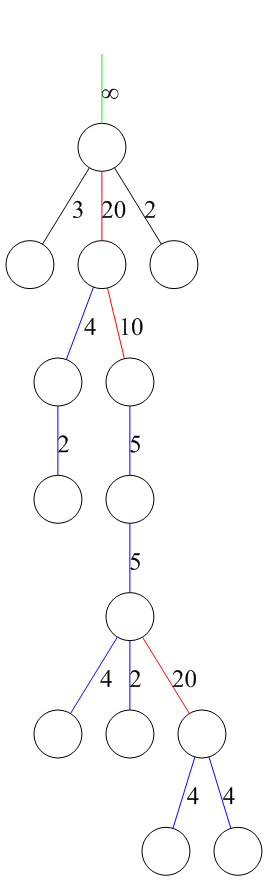
\includegraphics[width=.2\linewidth]{segmentation/segmentation-waterfall-nicholls-example-g.png}}%
	\hspace{4mm}%
	\subfigure[Result]{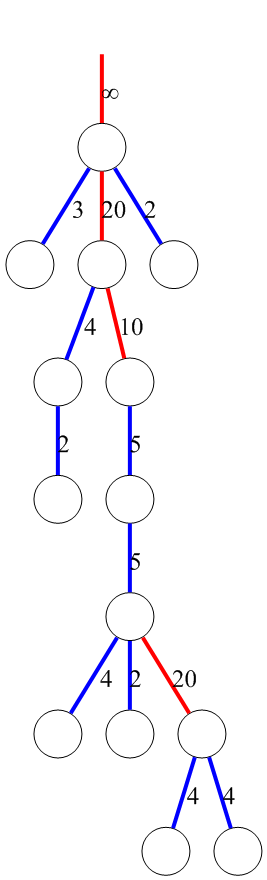
\includegraphics[width=.2\linewidth]{segmentation/segmentation-waterfall-nicholls-example-h.png}}%
\caption{Nicholls' algorithm in action (considering all the edges in each level at a time for space reasons): black edges are non-guards, red edges are guards, blue edges are those which have been elided and green edges are ones under active consideration.}
\label{fig:segmentation-waterfall-nicholls-example}
\end{stusubfig}
%---

The arbitrary assumption that all the implied flow is along the lowest child in the first case is this algorithm's way of dealing with non-minimal plateaux in the MST. It is a valid way of dealing with the problem (in that any choice here is arguably valid), but it is not robust: in particular, the selected direction of implied flow from a particular node depends on both where the MST is rooted, and the specific method used to choose the lowest child. It also ignores the possibility that part of the implied flow is along the parent. All of this fundamentally affects which edges are elided, and hence the result of the segmentation. In the following subsection, I will present an alternative tree-based algorithm which deals with this issue in a more robust manner.

\subsubsection{My Algorithm}
\label{subsubsec:segmentation-waterfall-myalgorithm}

Referring back to Meijster and Roerdink's image watershed algorithm in \S\ref{subsec:segmentation-watershed-greyscale}, we observe that one robust way of dealing with the problem of non-minimal plateaux in a landscape is to first transform the image to make it lower-complete: that is, we transform it into an image where every pixel that is not within a local minimum has a lower neighbour. The method for making the image lower-complete described in \cite{meijster98} has the effect of treating pixels which are further from the border of a plateau as being in some sense `higher' than those on the boundary. The same sort of idea can be applied in the context of a waterfall pass (although it is not necessary to actually transform the MST to make it lower-complete): where there are non-minimal plateaux in the MST, we can arrange to treat the nodes further from the border of the plateaux as being `higher' than their boundary counterparts. As we will see, this enables a robust decision to be made about which edges should be elided.

The proposed algorithm is a tree-based rainfalling method, and works in two recursive passes. The first pass works up the tree from the leaf nodes, marking initial path(s) of steepest descent from each node whilst allowing for the fact that they may need to be refined later. The second pass works down the tree from the root, updating the path(s) for each node to take account of routes via parent edges and eliding edges as necessary. The MST can be rooted anywhere in order to form the input tree -- the results are the same for any choice of root. In detail, the algorithm works as follows:

%-
\begin{enumerate}

\item \emph{Up Pass}. For each node, starting from the root:

%--
\begin{enumerate}

\item Recursively process any children (the fact that the children are processed first is the reason for this being called an `up' pass).

\item If this node has a unique edge of steepest descent (i.e.~a unique lowest-valued edge leading out of it, which can be the parent edge), add an arrow on the node pointing along the edge.

\item Otherwise, consider all the lowest-valued child edges (i.e.~ignore the parent for now, even if it is also a lowest-valued edge) which satisfy the condition that there is no arrow on the node at the other end of the edge pointing along the edge towards this node. If there are no such child edges, then this node is unescapable along a child edge and should be given a distance value of $\infty$. Otherwise, each of these child edges can be assigned a distance value equal to $1$ greater than the value on the node at the other end of the edge: this value on the node will be $0$ for nodes from which there is a unique path of steepest descent, and non-zero otherwise. Pick all the child edges whose distance value is minimal and add arrows to this node pointing along them (these indicate the initial paths of steepest descent from this node). Store the minimum distance value as this node's value.

\item Now consider the parent edge: if it was a lowest-valued edge, mark it as a potential path of steepest descent to avoid the need to check again in the second pass (in the diagram, an open-headed arrow is used to mark a parent edge for later processing).

\end{enumerate}
%--

\item \emph{Down Pass}. For each node, starting from the root:

%--
\begin{enumerate}

\item \emph{Check upwards route}. If a node was marked as having a potential upwards path of steepest descent, first check to make sure that there is no arrow on the parent node pointing down the edge to this node. If not, there is a possible route upwards whose distance value is $1$ greater than the value on the parent node. This is compared to any existing routes downwards via child edges. If the upwards route is strictly better, the downwards arrows are removed, the upwards route is marked and the distance value on the node is updated to reflect the better route. If the upwards route is equally good, the parent edge is marked but no other changes are made. If the upwards route is worse, it is simply ignored.

\item \emph{Check whether parent edge (if any) should be elided}. The decision on whether or not to elide an edge is based on a classification of its two end nodes with respect to the edge itself (this is why it can only be done at this point in the algorithm). Nodes can be classified into one of five types with respect to the edge: unambiguous in (the flow from the node goes only along this edge), ambiguous in (part, but not all, of the flow from the node goes along this edge), unambiguous out (the flow from the node goes along precisely one of the other edges leading out of it), ambiguous out (the flow from the node goes along at least two of the other edges leading out of it) and no flow (there is no flow from the node at all). Based on these classifications, the parent edge is either elided or not according to the case analysis shown in Figure~\ref{fig:segmentation-waterfall-smg-mergecases}. Note that there are only $13$ cases possible, rather than the expected $15$: \{ambiguous in, ambiguous in\} and \{ambiguous in, unambiguous in\} can never occur due to the way the algorithm works.

\item \emph{Recurse on any children}.

\end{enumerate}
%--

\end{enumerate}
%-

%---
\stufigex{width=.95\linewidth}{segmentation/segmentation-waterfall-smg-mergecases.png}{Case analysis for the edge elision step of my waterfall algorithm (a blue edge indicates that the edge would be elided; a red edge indicates that it wouldn't)}{fig:segmentation-waterfall-smg-mergecases}{p}
%---

It is possible to perform a case analysis for the first pass and the route resolution step 2(a) as well (see Figures~\ref{fig:segmentation-waterfall-smg-pass1cases} and \ref{fig:segmentation-waterfall-smg-resolutioncases}), and this is helpful to clarify the workings of the algorithm. As illustrated in the diagram, there are six cases for the first pass: (a) the node has a unique path of steepest descent down a child edge; (b) the node has a unique path of steepest descent up the parent edge; (c) the node has more than one path of steepest descent (and the parent edge is not a possible path of steepest descent); (d) the node has more than one \emph{downwards} path of steepest descent (but the parent edge still needs to be considered); (e) there is no flow out of the node and (f) there is no downwards flow out of the node (but the parent edge still needs to be considered). For the resolution step, there are four cases: (a) the arrow from the parent node points towards us; (b) there is no flow from the parent node; (c) there is an equally good route via the parent node and (d) there is a better route via the parent node. Figure~\ref{fig:segmentation-waterfall-smg-example} illustrates how the algorithm works on the now familiar graph used to demonstrate the workings of the previous two waterfall approaches.

%---
\begin{stusubfig}{p}
	\subfigure[The node has a unique path of steepest descent down a child edge]
	{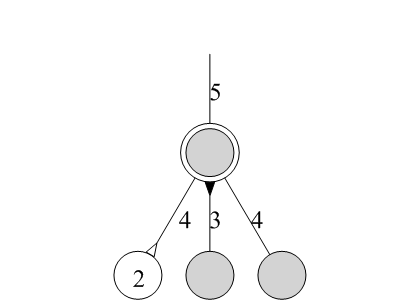
\includegraphics[width=.45\linewidth]{segmentation/segmentation-waterfall-smg-pass1cases-a.png}}%
	%
	\hspace{4mm}%
	%
	\subfigure[The node has a unique path of steepest descent up the parent edge]
	{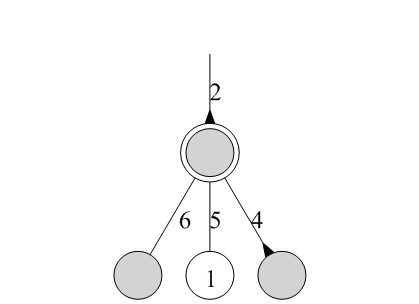
\includegraphics[width=.45\linewidth]{segmentation/segmentation-waterfall-smg-pass1cases-b.png}}%
	%
	\hspace{4mm}%
	%
	\subfigure[The node has more than one path of steepest descent (and the parent edge is not a possible path of steepest descent)]
	{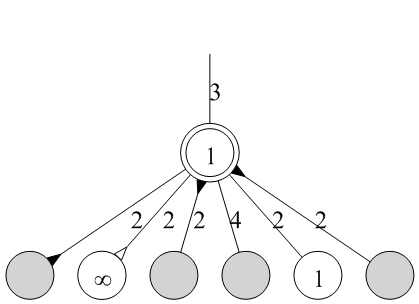
\includegraphics[width=.45\linewidth]{segmentation/segmentation-waterfall-smg-pass1cases-c.png}}%
	%
	\hspace{4mm}%
	%
	\subfigure[The node has more than one \emph{downwards} path of steepest descent (but the parent edge still needs to be considered)]
	{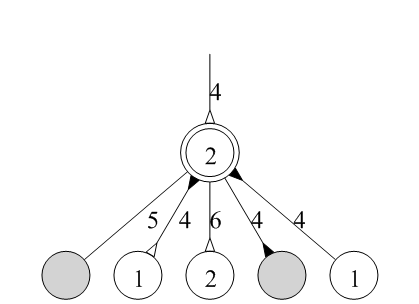
\includegraphics[width=.45\linewidth]{segmentation/segmentation-waterfall-smg-pass1cases-d.png}}%
	%
	\hspace{4mm}%
	%
	\subfigure[There is no flow out of the node]
	{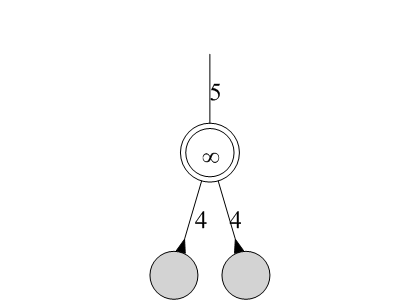
\includegraphics[width=.45\linewidth]{segmentation/segmentation-waterfall-smg-pass1cases-e.png}}%
	%
	\hspace{4mm}%
	%
	\subfigure[There is no downwards flow out of the node (but the parent edge still needs to be considered)]
	{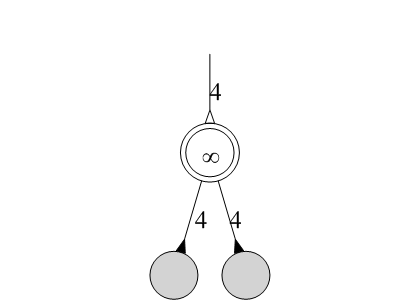
\includegraphics[width=.45\linewidth]{segmentation/segmentation-waterfall-smg-pass1cases-f.png}}%
\caption{Case analysis for the first pass of my waterfall algorithm}
\label{fig:segmentation-waterfall-smg-pass1cases}
\end{stusubfig}
%---

%---
\begin{stusubfig}{p}
	\subfigure[The arrow from the parent node points towards us]{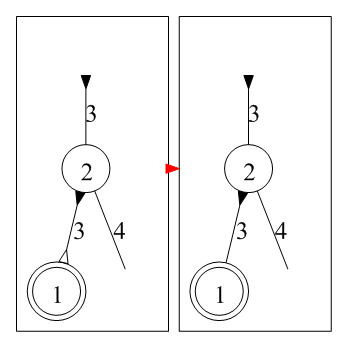
\includegraphics[height=5cm]{segmentation/segmentation-waterfall-smg-resolutioncases-a.png}}%
	%
	\hspace{4mm}%
	%
	\subfigure[There is no flow from the parent node]{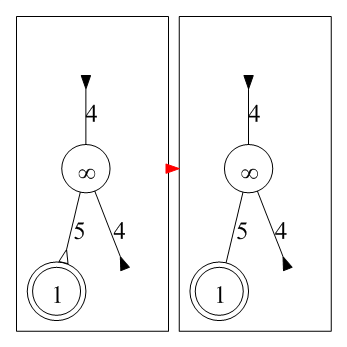
\includegraphics[height=5cm]{segmentation/segmentation-waterfall-smg-resolutioncases-b.png}}%
	%
	\hspace{4mm}%
	%
	\subfigure[There is an equally good route via the parent node]{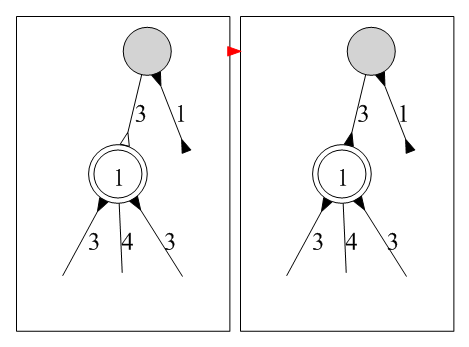
\includegraphics[height=5cm]{segmentation/segmentation-waterfall-smg-resolutioncases-c.png}}%
	%
	\hspace{4mm}%
	%
	\subfigure[There is a better route via the parent node]{\includegraphics[height=5cm]{segmentation/segmentation-waterfall-smg-resolutioncases-d.png}}%
\caption{Case analysis for the resolution step of my waterfall algorithm}
\label{fig:segmentation-waterfall-smg-resolutioncases}
\end{stusubfig}
%---

%---
\begin{stusubfig}{p}
	\subfigure[The initial tree]{\includegraphics[width=.3\linewidth]{segmentation/segmentation-waterfall-smg-example-initial.png}}%
	\hspace{4mm}%
	\subfigure[After the first pass]{\includegraphics[width=.3\linewidth]{segmentation/segmentation-waterfall-smg-example-pass1.png}}%
	\hspace{4mm}%
	\subfigure[The final result]{\includegraphics[width=.3\linewidth]{segmentation/segmentation-waterfall-smg-example-pass2.png}}%
\caption{My waterfall algorithm running on a real example: the arrows on the nodes indicate the flow direction, blue edges are those that are elided and red edges are those that aren't.}
\label{fig:segmentation-waterfall-smg-example}
\end{stusubfig}
%---

\subsubsection{Comparison}

Each of the three waterfall algorithms just described has different properties which may make it more or less suitable to use for a given application. The key issues to consider for each algorithm are: (a) the complexity of the algorithm, (b) how easy the algorithm is to implement and (c) the nature of the resulting output, in particular regarding the robustness of the algorithm with respect to changes in implementation details. A comparison of the algorithms is presented for each of these factors.

\paragraph{Complexity}

The complexity of all three algorithms tends to be (and, in the case of both Nicholls' algorithm and my algorithm, definitely is) dominated by the construction of a minimum spanning tree for the region adjacency graph of the initial partition. As of the time of writing, the fastest known algorithm for constructing a minimum spanning tree is Chazelle's algorithm \cite{?}, which is $O(E \; \alpha(E,V))$ (where $E$ is the number of edges in the graph, $V$ is the number of vertices and $\alpha$ is the functional inverse of the Ackermann function, which grows incredibly slowly). Most normal implementations, however, are likely to either use Kruskal's algorithm ($O(E \log V)$ as most commonly implemented) or Prim's algorithm ($O(E + V \log V)$ using a Fibonnaci heap).

All three algorithms converge to a partition with a single region in a very small number of iterations, so for practical purposes the number of iterations necessary can be treated as being $\Theta(1)$.

\subparagraph{Marcotegui's Algorithm}

The complexity of the implementation of Marcotegui's algorithm suggested when it was described above is somewhat hard to characterise, due to the flooding process proposed for the implementation of step 1 of each iteration (determining the local minima of the MST). However, an iteration of Marcotegui's algorithm can be implemented in an entirely equivalent manner by running my waterfall algorithm on the MST to perform step 1: this classifies the edges of the MST (see Figure~\ref{fig:segmentation-waterfall-smg-mergecases}), allowing those edges which form the MST's local minima to simply be read off. In particular, the edges we are interested in are those classified as either (a) \{unambiguous in, unambiguous in\} -- a singular minimum, (b) \{unambiguous in, no flow\} -- on the boundary of a minimal plateau, or (c) \{no flow, no flow\} -- within a minimal plateau. As will be shown via the complexity analysis of my algorithm below, these can all be determined in $\Theta(V)$ time. The edges can then be directly elided in $O(V)$ time in step 2 (note that it is unnecessary to separate them into their respective local minima, since they are all to be elided).

The analysis of the propagation process in step 3 depends on the implementation of the priority queue. Assuming the common heap-based approach \cite{clr-pq} is used, both the insertion and extraction operations on the priority queue are logarithmic in complexity. We can then observe that all the edges of the MST which did not form part of a local minimum are inserted into the priority queue once only and later extracted. Since there are (by definition) $V - 1$ edges in total in the MST, there are $O(V)$ such `non-minimal' edges, so the overall cost of the various logarithmic priority queue operations is $O(V \lg V)$. The elision performed on each edge after it is extracted is $\Theta(1)$, so the overall cost of the propagation step is $O(V \lg V)$. The complexity of an iteration of Marcotegui's algorithm is thus also $O(V \lg V)$, since the propagation step is the most costly part of the algorithm.

The overall complexity of Marcotegui's algorithm depends on which minimum spanning tree construction process is used. If either Kruskal's algorithm or Prim's algorithm is chosen, the complexity of that dominates the complexity of the actual iterations. Were Chazelle's algorithm to be implemented, however, the complexity of the overall algorithm would be $O(E \; \alpha(E,V) + V \lg V)$.

\subparagraph{Nicholls' Algorithm}

Each iteration of Nicholls' algorithm is $\Theta(V)$. To justify this, consider once more that there are by definition $V - 1$ edges in the MST, and that the algorithm accesses each edge a constant number of times. More specifically, each edge is processed itself, accessed again in the course of finding the lowest child of its parent, and then possibly accessed once more if it is to be elided.

The overall complexity of Nicholls' algorithm is the same as the complexity of the minimum spanning tree construction process (whichever MST algorithm is used), since the complexity of a constant number of iterations is still $\Theta(V)$, and all the MST algorithms are $\Omega(V)$, since the original graph was connected and so $E \in \Omega(V)$.

\subparagraph{My Algorithm}

Each iteration of my algorithm is also $\Theta(V)$. As before, we observe that there are $V - 1$ edges in the MST. Separate arguments can then be made for the up and down passes. For the up pass, note that each edge is considered a constant number of times (once as the child edge of a node in 1(b), once as the edge leading up from a node in 1(b), potentially once as a lowest-valued child edge in 1(c), and potentially once as a lowest-valued edge which was also the parent in 1(d)). The up pass as a whole is thus $\Theta(V)$. For the down pass, steps 2(a) and 2(b) involve a constant amount of work, and step 2(c) just implies that this is done for each node, so the overall amount of work is again $\Theta(V)$. A full iteration of the algorithm is thus also $\Theta(V)$.

The overall complexity of my algorithm is once again the same as the complexity of the minimum spanning tree construction process (whichever MST algorithm is used).

\paragraph{Ease of Implementation}

Of the three waterfall algorithms, Nicholls' algorithm is the easiest to implement: the iteration process itself can be implemented using a single, short, recursive function. It is particularly suitable for implementation in a functional language such as Haskell (this was a key motivation for its development), but is no harder to implement in imperative languages. My algorithm is slightly harder to implement, because it requires two separate passes over the tree for each iteration, but each pass is still simple and recursive. Marcotegui's algorithm is the hardest of the three to implement. If my algorithm is used to find the local minimum edges in preference to the flooding-based approach described earlier, however, the implementation is still relatively simple. All that is then required for each iteration is an implementation of the propagation step, which can be done straightforwardly using a priority queue, as already mentioned.

\paragraph{Nature of Output}

The key difference between the three algorithms presented is in the nature of their output. Although the algorithms exist to solve the same problem, they do not in general give precisely the same results. As discussed when motivating the development of my algorithm above, this is ultimately a result of different decisions as to how best to deal with non-minimal plateaux in the MST: Marcotegui's algorithm and Nicholls' algorithm take (different) implementation-dependent, implicit approaches to non-minimal plateaux, whilst mine accounts for them in a consistent, explicit manner. (This does not imply that my algorithm yields better results: rather, it yields more consistent results which do not depend on implementation choices. It is worth noting that the results of running the three different algorithms on an MST with no non-minimal plateaux are actually identical: the only difference occurs when non-minimal plateaux are present.)

The variation in output that can occur is most easily understood by comparing the output of the three algorithms on an example MST with a non-minimal plateau: see Figure~\ref{fig:segmentation-waterfall-comparison}. (Note that since both Marcotegui's algorithm and Nicholls' algorithm can produce different results based on specific implementation details, only one of the possible results is shown for each.) There are a number of important things to observe:
%
\begin{enumerate}

\item Whilst Marcotegui's algorithm and Nicholls' algorithm produce results which contain the same number of regions (the number of regions produced in each case is equal to the number of local minima in the MST), my algorithm may produce a result containing more regions than the other algorithms, because it avoids making an arbitrary merging decision in ambiguous situations. This was a deliberate design choice made in the development of my algorithm: it would be easy enough to change the algorithm to instead arbitrarily pick one of the possible directions of flow from an ambiguous node in step 2(b) of my algorithm if desired.

\item The output from Nicholls' algorithm could have been generated by Marcotegui's algorithm had the order of edge extraction from the priority queue in the latter been different. The converse is also true, were the MST to be rooted at a different node. Note, however, that when faced with an ambiguous node of the type shown (the one labelled with a 1 in the result from my algorithm), Nicholls' algorithm will always choose to keep the parent edge.

\item My algorithm produces the same result regardless of where the MST is rooted.

\end{enumerate}
%

%---
\begin{stusubfig}{p}
	\subfigure[The input MST]
	{\includegraphics[width=.4\linewidth]{segmentation/segmentation-waterfall-comparison-input.png}}%
	\hspace{4mm}%
	\subfigure[A possible Marcotegui's algorithm result]
	{\includegraphics[width=.4\linewidth]{segmentation/segmentation-waterfall-comparison-marcotegui.png}}%
	\\
	\subfigure[A possible Nicholls' algorithm result]
	{\includegraphics[width=.4\linewidth]{segmentation/segmentation-waterfall-comparison-nicholls.png}}%
	\hspace{4mm}%
	\subfigure[The result of my algorithm]
	{\includegraphics[width=.4\linewidth]{segmentation/segmentation-waterfall-comparison-smg.png}}%
\caption{Comparing the outputs of the three different waterfall algorithms on a sample MST with a non-minimal plateau.}
\label{fig:segmentation-waterfall-comparison}
\end{stusubfig}
%---

\paragraph{Summary}

Having compared the three waterfall algorithms in terms of their algorithmic complexity, ease of implementation, and output, it is possible to draw some conclusions about when it is more appropriate to choose one over another. If ease of implementation is the primary consideration for an application, and the details of how non-minimal plateaux should be handled are unimportant, then Nicholls' algorithm is the best approach. If, however, non-minimal plateaux need to be handled consistently, my algorithm is a more appropriate choice.

%---
\section{IPF Construction}
\label{sec:segmentation-ipfconstruction}

TODO (don't forget to discuss the effects of using different pre-processing approaches)

\subsection{Overview}

Having now seen how the watershed and waterfall transforms can be implemented, it remains to demonstrate how they can be used to construct an image partition forest as defined in the previous chapter. The first step is illustrate the sort of IPF we want to create (see Figure~\ref{fig:segmentation-ipfconstruction-goal}). The leaf layer corresponds directly to the original image, in that each node in it corresponds to a pixel in the image. The branch layers represent partitions of the image that become increasingly coarse as we ascend the forest. (Of course, the leaf layer is itself a partition of the image, if a trivial one.)

% TODO: fig:segmentation-ipfconstruction-goal

We observe that the watershed process described produces an initial (relatively fine) partition of the image, which is then iteratively refined by the waterfall to give a sequence of ever coarser partitions. The idea, therefore, is that the lowest branch layer of the forest will correspond to the initial partition of the image output by the watershed, with higher branch layers being created by the waterfall.

\subsubsection{Region Properties}

\paragraph{Discussion}

As per the description of IPFs in the previous chapter, it is possible to associate properties with forest nodes that in some way describe the regions they represent. We can use this to provide necessary information to feature identification algorithms, in particular those that will be described in the next chapter. (As a simple example, such algorithms might look for regions whose mean grey value was greater than a certain threshold, and we might arrange for a mean grey value property to be calculated for each region to support this.)

The decision about which properties to provide evidently depends on the feature identification algorithms in use. For the IPF algorithms to work, however, we have to bear in mind that it must be possible to calculate the set of properties for a particular node from the properties of its children. We will see that for certain properties (such as elongatedness), it may be necessary to augment the set of properties chosen in order to provide sufficient information in the properties of the children for this to be possible.

It is not necessary, however, for nodes in every layer to have the same set of properties: the ability to combine the properties of the various children of a node to obtain the properties of the node itself is sufficient. For our application, this allows us to make a space optimization for the leaf layer, whose many nodes represent individual pixels in the image. For these nodes, there is no need to store e.g.~properties such as the area of the represented region, since it is trivially $1$ for every node in the layer. When calculating the properties of the lowest branch layer from its children in the leaf layer, it is easy enough to treat the children as having an area of $1$, without needing to explicitly store it anywhere.

\paragraph{Chosen Property Sets}

For the feature identification algorithms in Chapter~\ref{chap:featureid}, at least, the properties needed for leaf nodes are:

\begin{itemize}

\item \emph{Feature ID}. One of an application-specific set of possible labels. The set used here is: \{None, Aorta, Inferior Vena Cava, Left Kidney, Liver, Other Artery, Other Vein, Rib, Right Kidney, Spinal Cord, Spine, Spleen, Tumour (Necrotic), Tumour (Normal)\}. Initially set to `None', prior to identifying any image features.

\item \emph{Grey Value}. The value of the pixel in the grey value image that results from applying a CT windowing transformation to the original Hounsfield image.

\item \emph{Hounsfield Value}. The original Hounsfield Unit (HU) value of the pixel.

\end{itemize}

\noindent For branch nodes, the necessary properties are:

\begin{itemize}
\item \emph{Area}. The area of the region, in pixels.
\item \emph{Central Moments}. TODO
\item \emph{Centroid}. The centre of the region, as a vector $\in \mathbb{R}^3$.
\item \emph{Elongatedness}. TODO
\item \emph{Feature ID}. As above.
\item \emph{Grey Value Max}. The maximum grey value of a pixel in the region.
\item \emph{Grey Value Mean}. The mean grey value of a pixel in the region, as a scalar $\in \mathbb{R}$.
\item \emph{Grey Value Variance}. The variance of the distribution of grey values for all pixels in the region.
\item \emph{Hounsfield Value Max}. The maximum HU value of a pixel in the region.
\item \emph{Hounsfield Value Mean}. The mean HU value of a pixel in the region.
\item \emph{Hounsfield Value Variance}. The variance of the HU distribution for all pixels in the region.
\end{itemize}

\noindent It is necessary to show how properties for several leaf nodes can be combined to determine the properties of their (branch node) parent, and how properties of several branch nodes can likewise be combined.

TODO

\subsection{Constructing the Lowest Two Layers}

TODO

\subsection{Constructing the Higher Layers}

TODO

%---
\section{Chapter Summary}

In this chapter, we saw how to generate IPFs from medical images using the morphological watershed and waterfall transforms. The next chapter will show how the generated IPFs can be used to automatically identify salient features in the original images.
